\documentclass[12pt,a4paper,twoside]{book}


% ==========================================================
% PACOTES
% ==========================================================
\usepackage{multicol}
\usepackage{fontspec}
\usepackage{etoolbox}
\usepackage{environ}
\usepackage{float}
\usepackage{witharrows}
\usepackage{eso-pic, pgf-pie}
\usepackage{pgfplots}
\usepackage{cancel}
\usepackage{tikz}
\usepackage{amsmath}
\usepackage{tcolorbox}
\tcbuselibrary{breakable}

\newcommand{\canceldiv}[2]{%
    \cancel{#1}^{\div #2}%
}

\renewcommand{\CancelColor}{\color{red}}

\usepackage{polyglossia}
\setmainlanguage{portuguese}
\setotherlanguage{english}

% Fonte
\setmainfont{TeX Gyre Heros}


% Matemática

\usepackage{unicode-math}

\setmathfont{Latin Modern Math}
% Layout
\usepackage[
    a4paper,
    top=2cm,
    bottom=2cm,
    left=1.5cm,
    right=2.0cm,
    headheight=15pt
]{geometry}

% TikZ
\usepackage{tikz}
\usetikzlibrary{
    calc,
    positioning,
    shapes.geometric,
    shapes.misc,
    arrows.meta,
    backgrounds,
    decorations.pathmorphing,
    fadings
}

% Caixas
\usepackage{tcolorbox}
\tcbuselibrary{
    skins,
    breakable
}

% Listas
\usepackage{enumitem}

% Links
\usepackage[
    colorlinks=true,
    linkcolor=AzulPrincipal,
    urlcolor=Roxo,
    citecolor=AzulPrincipal
]{hyperref}

% Cabeçalho
\usepackage{fancyhdr}

% Controle de títulos
\usepackage{titlesec}

% Espaçamento
\usepackage{setspace}
\setstretch{1.08}

% Imagens
\usepackage{graphicx}

% Tabelas
\usepackage{array}
\usepackage{booktabs}

% ==========================================================
% CONFIGURAÇÕES GERAIS
% ==========================================================

\setlength{\parindent}{0pt}
\setlength{\parskip}{6pt}

\setlist[itemize]{
    leftmargin=*,
    itemsep=2pt
}

\setlist[enumerate]{
    leftmargin=*,
    itemsep=4pt
}

% ==========================================================
% CABEÇALHO E RODAPÉ
% ==========================================================

\pagestyle{fancy}

\fancyhf{}

\fancyhead[LE]{
    \small\color{CinzaTexto}
    Banco de Questões de Matemática
}

\fancyhead[RO]{
    \small\color{CinzaTexto}
    \leftmark
}

\fancyfoot[C]{
    \tikz[baseline=-0.5ex]{
        \node[
            circle,
            fill=AzulPrincipal,
            text=white,
            minimum size=0.65cm,
            inner sep=0pt
        ] {\small\thepage};
    }
}

\renewcommand{\headrulewidth}{0pt}
\renewcommand{\footrulewidth}{0pt}


% ==========================================================
% CAPÍTULOS
% ==========================================================

\titleformat
{\chapter}
[display]
{\normalfont\sffamily}
{}
{0pt}
{%
    \begin{tikzpicture}[overlay]
        \node[
            fill=AzulPrincipal,
            text=white,
            rounded corners=8pt,
            inner xsep=15pt,
            inner ysep=5pt
        ] at (2.4,.3) {\Large\bfseries CAPÍTULO \thechapter};
    \end{tikzpicture}
    \hspace{5cm}
    \Huge\bfseries
}
[
    \vspace{-.9cm}
    \color{Turquesa}
    \rule{\textwidth}{3pt}
]


\titleformat
{name=\chapter,numberless}
[display]
{\normalfont\sffamily}
{}
{0pt}
{
    \Huge\bfseries
}
[
    \vspace{-1.1cm}
    \color{Turquesa}
    \rule{\textwidth}{3pt}
]

\titlespacing*{\chapter}
{0pt}{-20pt}{30pt}

% ==========================================================
% SEÇÕES
% ==========================================================

\titleformat
{\section}
{\Large\bfseries\sffamily\color{AzulPrincipal}}
{\thesection}
{0.7em}
{}

\titleformat
{\subsection}
{\large\bfseries\sffamily\color{Roxo}}
{\thesubsection}
{0.7em}
{}

% =============================================================
% AMBIENTE DE OBSERVAÇÃO OU DICAS
% =============================================================

\newtcolorbox{observacao}[1][Observação]{
    colback=VerdeDestaqueFundo,
    colframe=VerdeDestaque,
    boxrule=0pt,
    leftrule=4pt,
    arc=2pt,
    left=10pt,
    right=10pt,
    top=8pt,
    bottom=8pt,
    enhanced,
    before upper={%
        \textcolor{VerdeDestaque}{\textbf{#1}}
        \par\smallskip
    },
}
% ==========================================================
% PALETA DE CORES
% ==========================================================

\definecolor{AzulPrincipal}{HTML}{173F5F}
\definecolor{AzulClaro}{HTML}{20639B}
\definecolor{Turquesa}{HTML}{3CAEA3}
\definecolor{Verde}{HTML}{2A9D8F}
\definecolor{Amarelo}{HTML}{F6C85F}
\definecolor{Laranja}{HTML}{F4A261}
\definecolor{Vermelho}{HTML}{E76F51}
\definecolor{Roxo}{HTML}{6C63A8}
\definecolor{VerdeDestaque}{HTML}{3A9D5D}
\definecolor{VerdeDestaqueFundo}{HTML}{F0FAF2}

\definecolor{Fundo}{HTML}{F7F9FC}
\definecolor{CinzaTexto}{HTML}{4A5568}
\definecolor{CinzaClaro}{HTML}{E9EEF4}
\definecolor{VermelhoSolucao}{HTML}{C94C4C}
\definecolor{VermelhoSolucaoFundo}{HTML}{FDF2F2}
\definecolor{TurquesaTeorema}{HTML}{159A9C}
\definecolor{TurquesaTeoremaFundo}{HTML}{F0FAFA}

% ==========================================================
% CAIXA DE QUESTÃO
% ==========================================================

\newtcolorbox{caixaquestao}{
    enhanced,
    breakable,
    colback=white,
    colframe=CinzaClaro,
    boxrule=0.7pt,
    arc=8pt,
    left=12pt,
    right=12pt,
    top=12pt,
    bottom=12pt,
    before skip=12pt,
    after skip=18pt,
    borderline west={4pt}{0pt}{AzulPrincipal}
}

% ==========================================================
% CAIXA DE DESAFIO
% ==========================================================

\newtcolorbox{caixadesafio}{
    enhanced,
    breakable,
    colback=Amarelo!12,
    colframe=Amarelo!70!black,
    boxrule=0.8pt,
    arc=8pt,
    left=14pt,
    right=14pt,
    top=12pt,
    bottom=12pt,
    title={\sffamily\bfseries DESAFIO},
    coltitle=AzulPrincipal,
    fonttitle=\bfseries
}

% ==========================================================
% CAIXA DE DICA
% ==========================================================

\newtcolorbox{caixadica}{
    enhanced,
    breakable,
    colback=Turquesa!8,
    colframe=Turquesa,
    boxrule=0.7pt,
    arc=8pt,
    left=14pt,
    right=14pt,
    top=10pt,
    bottom=10pt,
    title={\sffamily\bfseries DICA},
    coltitle=AzulPrincipal,
    fonttitle=\bfseries
}

% ==========================================================
% CAIXA DE INFORMAÇÃO
% ==========================================================

\newtcolorbox{caixainfo}{
    enhanced,
    breakable,
    colback=AzulPrincipal!5,
    colframe=AzulPrincipal,
    boxrule=0.7pt,
    arc=8pt,
    left=14pt,
    right=14pt,
    top=10pt,
    bottom=10pt
}

% ==========================================================
% COMANDO PARA NÍVEL
% ==========================================================

\newcommand{\nivel}[1]{
    \textcolor{CinzaTexto}{\small\textbf{Nível: }}
    \foreach \n in {1,...,3}{
        \ifnum\n<#1+1
            \textcolor{Laranja}{\Large$\bullet$}
        \else
            \textcolor{CinzaClaro}{\Large$\bullet$}
        \fi
    }
}

% ==========================================================
% IDENTIFICAÇÃO DA QUESTÃO
% ==========================================================

\newcommand{\cabecalhoquestao}[2]{
    \begin{tikzpicture}
        \node[
            circle,
            fill=AzulPrincipal,
            text=white,
            minimum size=0.85cm,
            inner sep=0pt,
            font=\bfseries
        ] {#1};

        \node[
            anchor=west,
            font=\small\sffamily\bfseries,
            text=AzulPrincipal
        ] at (0.6cm,0) {QUESTÃO};

        \node[
            anchor=west,
            font=\small\sffamily,
            text=CinzaTexto
        ] at (2.0cm,0) {#2};
    \end{tikzpicture}
}

% ==========================================================
% QUESTÃO
% ==========================================================

\newcounter{questao}

\newcommand{\questao}[3]{
    \stepcounter{questao}

    \begin{caixaquestao}

        \cabecalhoquestao{\thequestao}{#1}

        \vspace{8pt}

        #2

        \vspace{8pt}

        #3

    \end{caixaquestao}
}

% ==========================================================
% ALTERNATIVAS
% ==========================================================

\newenvironment{alternativas}{
    \begin{enumerate}[
        label=\textbf{\Alph*)},
        labelsep=0.5em,
        itemsep=5pt
    ]
}{
    \end{enumerate}
}

% ==========================================================
% IDENTIFICAÇÃO PEDAGÓGICA
% ==========================================================

\newcommand{\metadados}[3]{
    \vspace{5pt}

    \begin{tikzpicture}
        \node[
            fill=AzulPrincipal!7,
            rounded corners=5pt,
            inner xsep=8pt,
            inner ysep=4pt,
            text=AzulPrincipal,
            font=\scriptsize\sffamily
        ] {
            \textbf{Conteúdo:} #1
            \hspace{10pt}
            \textbf{Habilidade:} #2
            \hspace{10pt}
            \textbf{#3}
        };
    \end{tikzpicture}
}

% ==============================================================
% CAIXA SOLUÇÃO
% ==============================================================

\newtcolorbox{caixasolucao}{
    colback=VermelhoSolucaoFundo,
    colframe=VermelhoSolucao,
    boxrule=0pt,
    leftrule=3pt,
    arc=2pt,
    left=8pt,
    right=8pt,
    top=8pt,
    bottom=8pt,
    enhanced,
    breakable,
}

% ==================================================================
% CAIXA TEOREMA
% ==================================================================

\newtcolorbox{Teorema}[1]{
    colback=TurquesaTeoremaFundo,
    colframe=TurquesaTeorema,
    boxrule=0pt,
    leftrule=4pt,
    arc=2pt,
    left=10pt,
    right=10pt,
    top=8pt,
    bottom=8pt,
    enhanced,
    before upper={%
        \textcolor{TurquesaTeorema}{\textbf{Teorema — #1}}
        \par\smallskip
    },
}
% ============================================================
% CAPÍTULOS SEM NUMERAÇÃO
% ============================================================

\newcommand{\capitulopreliminar}[1]{%
    \cleardoublepage
    \chapter*{#1}
    \addcontentsline{toc}{chapter}{#1}
    \markboth{#1}{#1}
}

% ==========================================================
% TEOREMAS
% ==========================================================


% ==========================================================
% ARMAZENAMENTO DE SOLUÇÃO
% ==========================================================

\newcounter{contsolucao}

\newenvironment{solucoes}[1]{%
    \setcounter{contsolucao}{0}%
    \def\totalSolucoes{#1}%
    \par\medskip
}{%
    \ifnum\value{contsolucao}>0
        \end{caixasolucao}
    \fi
    \par\medskip
}

% ==================================================
% COMANDO DE SOLUÇÃO
% ==================================================

\newcommand{\solucao}{%
    \ifnum\value{contsolucao}>0
        \end{caixasolucao}
    \fi
    \stepcounter{contsolucao}%
    \begin{caixasolucao}
    \textbf{\textcolor{VermelhoSolucao}{Solução%
        \ifnum\totalSolucoes>1
            \space
            \ifnum\value{contsolucao}<10
                0%
            \fi
            \arabic{contsolucao}%
        \fi
    }}%
    \par\smallskip
}
% ==================================================
% CONTADOR DE QUESTÕES
% ==================================================

\newcounter{numeroquestao}

\renewcommand{\thenumeroquestao}{%
    \ifnum\value{numeroquestao}<10
        0\arabic{numeroquestao}%
    \else
        \arabic{numeroquestao}%
    \fi
}

\makeatletter

\let\sectionoriginal\section

\renewcommand{\section}{%
    \@ifstar
        {\sectionsemnumero}
        {\sectioncomnumero}%
}

\newcommand{\sectioncomnumero}[1]{%
    \setcounter{numeroquestao}{0}%
    \sectionoriginal{#1}%
}

\newcommand{\sectionsemnumero}[1]{%
    \setcounter{numeroquestao}{0}%
    \sectionoriginal*{#1}%
}

\makeatother

% ============================================================
% ESTILO DAS QUESTÕES
%=============================================================

\renewcommand{\questao}[1]{%
    \refstepcounter{numeroquestao}
    \noindent
    \hangindent=0cm
    \hangafter=-1
    \makebox[2.85cm][l]{
    
\begin{tikzpicture}[baseline=-.25cm]
        \node[
            fill=AzulPrincipal,
            text=white,
            rounded corners=3pt,
            minimum width=1cm,
            minimum height=0.8cm,
            font=\bfseries
        ] (numero) {Questão \thenumeroquestao};
        \draw[
            Turquesa,
            line width=2pt
        ]
        ([xshift=.3cm, yshift=.37cm]numero.east) -- ++(\dimexpr\textwidth-2.95cm\relax,0);
        
    \end{tikzpicture}%
    }
    #1
    \par 
    \vspace{.3cm}
    }


% =====================================================================
% PÁGINA DEDICADA AOS AUTORES
% =====================================================================

\newcommand{\paginaautores}{%
    \cleardoublepage
    \thispagestyle{empty}

    \begin{center}

        \vspace*{1cm}

        {\Large\bfseries\color{AzulPrincipal}
        AUTORES}

        \vspace{0.3cm}

        {\color{Turquesa}\rule{5cm}{2pt}}

        \vspace{1.2cm}

        % Autor 1
        {\large\bfseries\color{AzulPrincipal}
        Jadiel José Araújo da Silva Júnior}

        \vspace{0.2cm}

        {\normalsize
        Licenciado em Matemática - UFAL\\
        Mestre em Matemática - UFAL}

        \vspace{1cm}

        % Autor 2
        {\large\bfseries\color{AzulPrincipal}
        Samuel de Sousa Apolinário}

        \vspace{0.2cm}

        {\normalsize
        Licenciado em Matemática - UNEAL\\
        Especialista em Estatística Aplicada - FFOCUS\\
        Especialista em Matemática Orientada a Computação Gráfica - FFOCUS}

        \vspace{1cm}

        % Autor 3
        {\large\bfseries\color{AzulPrincipal}
        Gabriel Dória de Mendonça}

        \vspace{0.2cm}

        {\normalsize
        Licenciado em Matemática - UFAL}

        \vfill

        {\color{Turquesa}\rule{5cm}{1pt}}

        \vspace{0.3cm}

        {\small
        Banco de Questões de Matemática}

    \end{center}

    \cleardoublepage
}


\begin{document}

\frontmatter

\begin{titlepage}

\begin{tikzpicture}[remember picture,overlay]

% Fundo
\fill[Fundo]
    (current page.south west)
    rectangle
    (current page.north east);

% Faixa azul
\fill[AzulPrincipal]
    (current page.north west)
    rectangle
    ([xshift=0.38\paperwidth]current page.south west);

% Círculos decorativos
\fill[Turquesa]
    ([xshift=0.25\paperwidth,yshift=-2cm]current page.north west)
    circle (3cm);

\fill[Laranja]
    ([xshift=0.32\paperwidth,yshift=-7cm]current page.north west)
    circle (1.5cm);

\fill[Roxo]
    ([xshift=0.20\paperwidth,yshift=-11cm]current page.north west)
    circle (2.2cm);

% Triângulo
\node[
    regular polygon,
    regular polygon sides=3,
    fill=Amarelo,
    minimum size=4cm,
    rotate=25
] at ([xshift=0.28\paperwidth,yshift=-15cm]current page.north west) {};

% Hexagono
\node[
    regular polygon,
    regular polygon sides=7,
    fill=cyan,
    minimum size=4cm,
    rotate=25
] at ([xshift=0.1\paperwidth,yshift=-19cm]current page.north west) {};

ires
% Símbolos matemáticos
\node[
    text=white,
    font=\fontsize{38}{40}\selectfont
] at ([xshift=0.19\paperwidth,yshift=-4cm]current page.north west) {$\sum$};

\node[
    text=white,
    font=\fontsize{32}{35}\selectfont
] at ([xshift=0.12\paperwidth,yshift=-8cm]current page.north west) {$\pi$};

\node[
    text=white,
    font=\fontsize{30}{35}\selectfont
] at ([xshift=0.28\paperwidth,yshift=-19cm]current page.north west) {$\sqrt{x}$};

\node[
    text=white,
    font=\fontsize{30}{35}\selectfont
] at ([xshift=0.13\paperwidth,yshift=-23cm]current page.north west) {$\int{}$};

\end{tikzpicture}

\vspace*{3cm}

\hspace*{0.42\textwidth}
\begin{minipage}{0.57\textwidth}

{\color{AzulPrincipal}
\fontsize{17}{20}\selectfont
\bfseries BANCO DE QUESTÕES
}

\vspace{0.5cm}

{\color{AzulPrincipal}
\fontsize{38}{42}\selectfont
\bfseries MATEMÁTICA
}

\vspace{0.5cm}

{\color{CinzaTexto}
\Large
6º ao 9º ano do Ensino Fundamental
}

\vspace{1.5cm}

\begin{tcolorbox}[
    colback=white,
    colframe=Turquesa,
    boxrule=1pt,
    arc=8pt
]
\centering
\large
Questões organizadas por\\
\textbf{Unidades Temáticas}
\end{tcolorbox}

\vspace{10cm}

{\color{CinzaTexto}
\large
Organizadores
\vspace{30pt}

Prof. Me. Jadiel José Araújo da Silva Júnior \\
Prof. Esp. Samuel de Sousa Apolinário \\
Prof. Gabriel Dória de Mendonça
}

\end{minipage}

\end{titlepage}

\cleardoublepage

\paginaautores

\chapter*{Apresentação}
\addcontentsline{toc}{chapter}{Apresentação}

\begin{caixainfo}

Este livro foi desenvolvido como um banco de questões de Matemática
para os anos finais do Ensino Fundamental.

O material contempla conteúdos do \textbf{6º ao 9º ano}, organizados
por ano escolar e pelas principais Unidades Temáticas da Matemática.

\end{caixainfo}

\vspace{1cm}

\textbf{Como o livro está organizado}

O livro está dividido em quatro grandes capítulos:

\begin{itemize}
    \item \textbf{Capítulo 1 — 6º ano}
    \item \textbf{Capítulo 2 — 7º ano}
    \item \textbf{Capítulo 3 — 8º ano}
    \item \textbf{Capítulo 4 — 9º ano}
\end{itemize}

Dentro de cada capítulo, as questões são organizadas pelas Unidades
Temáticas:

\begin{itemize}
    \item Números;
    \item Álgebra;
    \item Geometria;
    \item Grandezas e Medidas;
    \item Probabilidade e Estatística.
\end{itemize}

\begin{caixadica}

\textbf{Sugestão de uso}

O professor pode utilizar este banco para elaborar listas de exercícios,
atividades de revisão, avaliações, simulados e outras propostas
pedagógicas.

\end{caixadica}

\cleardoublepage

\cleardoublepage
\renewcommand{\contentsname}{Sumário}
\tableofcontents
\cleardoublepage

\mainmatter

% Questões do 6° ano
\chapter{6$^{\circ}$ Ano}

\begin{caixainfo}

\textbf{Matemática — 6$^{\circ}$ ano}

Neste capítulo estão reunidas questões destinadas ao 6$^{\circ}$ ano do Ensino Fundamental, organizadas de acordo com as Unidades Temáticas da BNCC.

\end{caixainfo}

\vspace{1cm}

\section*{Unidades Temáticas}

\begin{center}

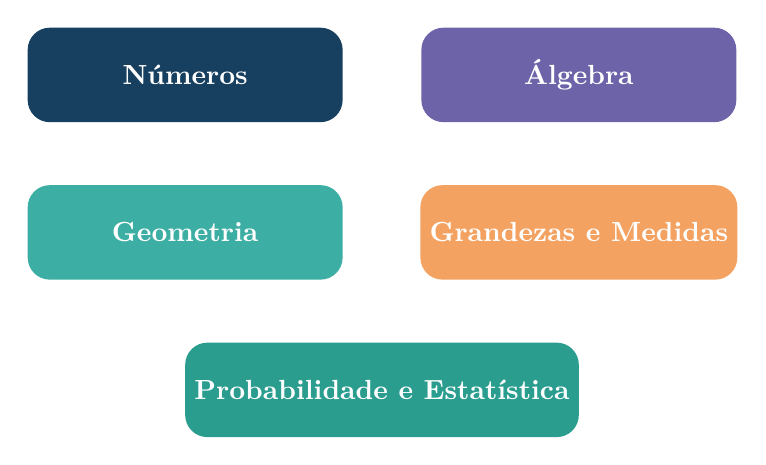
\begin{tikzpicture}

\node[
    rounded corners=8pt,
    fill=AzulPrincipal,
    text=white,
    minimum width=4cm,
    minimum height=1.2cm
] (n) at (0,0) {\textbf{Números}};

\node[
    rounded corners=8pt,
    fill=Roxo,
    text=white,
    minimum width=4cm,
    minimum height=1.2cm
] (a) at (5,0) {\textbf{Álgebra}};

\node[
    rounded corners=8pt,
    fill=Turquesa,
    text=white,
    minimum width=4cm,
    minimum height=1.2cm
] (g) at (0,-2) {\textbf{Geometria}};

\node[
    rounded corners=8pt,
    fill=Laranja,
    text=white,
    minimum width=4cm,
    minimum height=1.2cm
] (m) at (5,-2) {\textbf{Grandezas e Medidas}};

\node[
    rounded corners=8pt,
    fill=Verde,
    text=white,
    minimum width=4cm,
    minimum height=1.2cm
] (p) at (2.5,-4) {\textbf{Probabilidade e Estatística}};

\end{tikzpicture}

\end{center}

\clearpage


\section{Números}

\questao{A diretora Sheyla tem uma calculadora diferente das demais. Sua calculadora não possui teclas de operações e em seu lugar tem-se teclas com as letras E, M, S e P. Cada tecla possui uma habilidade:}
E - Pega o número colocado na tela e multiplica por 6 e subtrai dois 
\begin{figure}[htbp]
  \centering
  % Coluna da esquerda: Imagem
  \begin{minipage}{0.3\textwidth}
    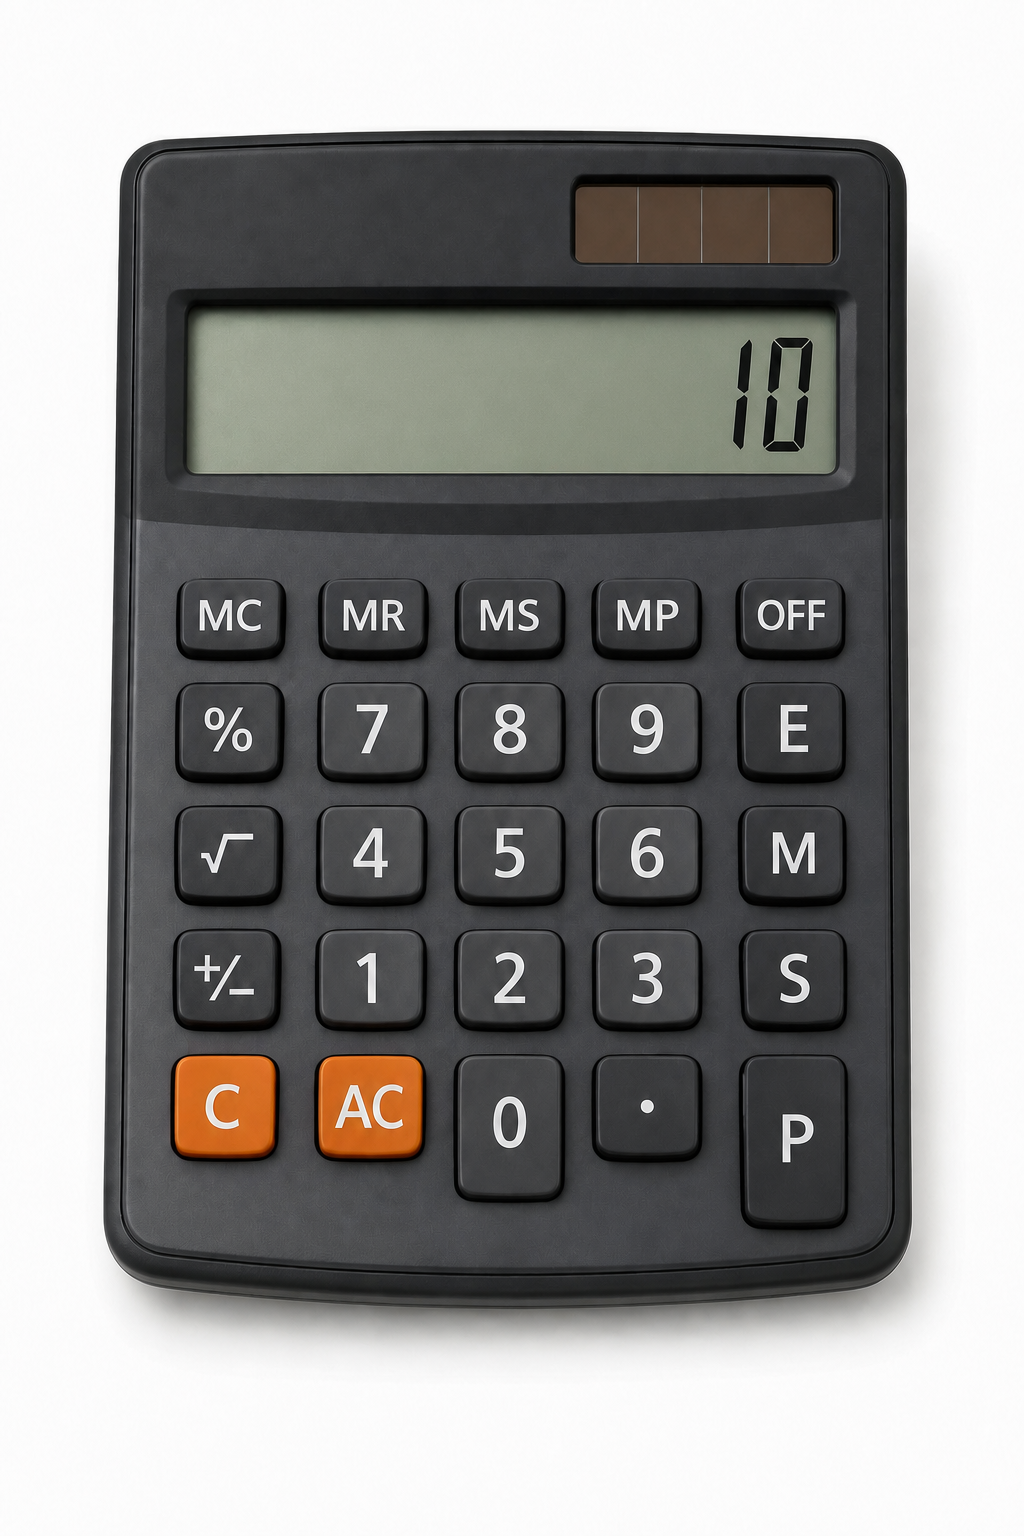
\includegraphics[width=\textwidth]{figuras/6_ano/IMG_0914.png} % Substitua pelo nome do seu arquivo
    \label{fig:minha_foto}
  \end{minipage}
  \hfill % Preenche o espaço entre as duas colunas
  % Coluna da direita: Texto
  \begin{minipage}{0.6\textwidth}
    \begin{itemize}
            \item  A tecla $E$ faz com que o número que está na tela seja multiplicado por 6 e após isso o resultado é subtraído por dois.
            \item  A tecla $M$ faz com que o número que está na tela seja dividido por dois e após isso o resultado é subtraído por cinco
            \item A tecla $S$ faz com que o número que está na tela permaneça o mesmo.
            \item A tecla $P$ faz com que o número que está na tela se transforme em zero.
        \end{itemize}
  \end{minipage}
\end{figure}
\begin{enumerate}[label=\alph*)]
    \item Na tela da calculadora da diretora Sheyla tem-se o número 10, igual a imagem da calculador. Se ela apertar em seguidas as teclas $E-M-P$, qual será o resultado apresentado na tela?
   
    \item Na tela da calculadora da diretora Sheyla tem-se o número 10, igual a imagem da calculador. Se ela apertar em seguidas as teclas $E-E-S-P-S-P$, qual será o resultado apresentado na tela?
    
    \item Na tela da calculadora da diretora Sheyla tem-se o número 10, igual a imagem da calculador. Se ela apertar em seguidas as teclas $E-E-E-S-M-S-E$, qual será o resultado apresentado na tela?
\end{enumerate}

\begin{solucoes}{1}
    \solucao
    \textbf{item a)}

    Para resolvermos o item a) é preciso observarmos apenas o último comando. Se observarmos a pergunta, a última tecla apresentada é a tecla $P$ que tem como função transformar o número da tela em 0. Logo, independentemente do que fizermos antes, o resultado final será 0. 

    \solucao
    \textbf{item b)}
    
       Para resolvermos o item b) é preciso observarmos apenas o último comando. Se observarmos a pergunta, a última tecla apresentada é a tecla $P$ que tem como função transformar o número da tela em 0. Logo, independentemente do que fizermos antes, o resultado final será 0 (Perceba que a quantidade de operações foi maior apenas para ver o nível de leitura, interpretação e estratégia de quem tentar resolvê-la).

\solucao
\textbf{item c)}

No item c) é preciso que se faça a série de execuções que se pedem. Na tela temos o número 10 e assim, fazendo $E-E-E-S-M-S-E$
\begin{equation*}
    10\cdot 6=60-2=58
\end{equation*}
\begin{equation*}
    58\cdot6=348-2=346
\end{equation*}
\begin{equation*}
    346\cdot 6=2076-2=2074 
\end{equation*}
Como a letra $S$ repete o mesmo resultado vamos ao próximo passo
\begin{equation*}
    \frac{2074}{2}=1037-5=1032
\end{equation*}
Por fim, 
\begin{equation*}
    1032\cdot6=6192-2=6190             
\end{equation*}
Portanto, o resultado na tela será $6190$.
       
\end{solucoes}

\questao{(OAM 2025 - Nível 1) A professora Joyce escreveu no quadro todos os divisores positivos do número $2025$.
Sabendo que ela levou exatamente $3$ segundos para escrever cada divisor, quanto tempo, em segundos,
ela gastou para escrever apenas os divisores de $2025$ que são múltiplos de $3$?}

\begin{solucoes}{1}
    \solucao
    Ao fatorar o número $2025$,tem-se, \\
    
    \begin{tabular}{r|l}
        $2025$ & $5$ \\
         $405$ & $5$ \\
         $81$ & $3$ \\
         $27$ & $3$ \\ 
         $9$ & $3$ \\
         $3$ & $3$\\ \cline{2-2}
         $1$ & $5^2\cdot 3^4$
    \end{tabular}
\\\\
Logos, podemos determinar a quantidade de divisores do número $2025$,onde $(2+1)\cdot (4+1)=3\cdot5=15$. São $15$ divisores, onde temos,

\begin{equation*}
    D_{2025}= \left\{ 1,3,5,9,15,25,27,45,75,81,135,225,405,675,2025\right\}
\end{equation*}

Os números $ \left\{3,9,15,27,45,75,81,135, 225, 405,675,2025\right\}$ são divisores de $2025$ e múltiplos de $3$ e como ela levou $3s$ para escrever cada um, temos $12\cdot 3=36s$.     
\end{solucoes}

\questao{(OAM 2025 - Nível 1) Um número é adoisado quando ele pode ser obtido pela soma de duas potências de $2$.
Por exemplo, $12$ é adoisado porque $12 =2^3 + 2^2$. Quantos números adoisados menores do que 1000
existem?}

\begin{solucoes}{2}
\solucao
Podemos separar em dois casos, potências iguais e potências diferentes. 

$i)$ Se as potências forem iguais, temos $9$ possibilidades, pois. $2^9+2^9=1024$ que é maior que $1000$.

$ii)$ Se as potências forem diferentes, temos $10$ possibilidades para a primeira escolha e $9$ para a segunda, logo $10\cdot 9=90$. Todavia, $2^8+2^9=2^9+2^8$ e assim precisamos dividir por dois para não contarmos duas vezes $\frac{90}{2}=45$.

Sendo assim, o total de números adoisados é $9+45=54$.
    
    \solucao
Sabemos que um número é adoisado quando ele pode ser obtido pela soma de duas potências de $2$ e queremos determinar a quantidade de números adoisados menores que $1000$. Até 1000 temos as potências $2^0=1$, $2^1=2$, $2^2=4$, $2^3=8$, $2^4=16$, $2^5=32$, $2^6=64$, $2^7=128$, $2^8=256$ e $2^9=512$, pois $2^{10}=1024$ que passa de $1000$. Logo, temos 10 números para serem somados. Vamos fixar um e variar os outros e descobriremos todos os casos,
\\\\
$1)$ Fixemos o $2^0=1$ e temos $10$ números que são adoisados. 
\\\\
$2)$ Fixemos o $2^1=2$ e tiremos os números $3=2^0+2^1$ que já foi computado no primeiro caso e assim temos $9$ números adoisados. 
\\\\
$3)$ Fixemos  o $2^2=4$ e tiremos os números $5=2^0+2^2$ e $6=2^1+2^2$ que já foram computados nos casos anteriores e assim temos $8$ números adoisados.
\\\\
$4)$ Fixemos  o $2^3=8$ e tiremos os números $9=2^0+2^3$, $10=2^1+2^3$ e $12=2^2+2^3$ que já foram computados nos casos anteriores e assim temos $7$ números adoisados.
\\\\
$5)$ Fixemos  o $2^4=16$ e tiremos os números $17=2^0+2^4$, $18=2^1+2^4$, $20=2^2+2^4$ e $24=2^3+2^4$ que já foram computados nos casos anteriores e assim temos $6$ números adoisados.
\\\\
$6)$ Fixemos  o $2^5=32$ e tiremos os números $33=2^0+2^5$, $34=2^1+2^5$, $36=2^2+2^5$, $40=2^3+2^5$ e $48=2^4+2^5$ que já foram computados nos casos anteriores e assim temos $5$ números adoisados.
\\\\
$7)$ Fixemos  o $2^6=64$ e tiremos os números $65=2^0+2^6$, $66=2^1+2^6$, $68=2^2+2^6$, $72=2^3+2^6$, $80=2^4+2^6$ e $96=2^5+2^6$ que já foram computados nos casos anteriores e assim temos $4$ números adoisados.
\\\\
$8)$ Fixemos  o $2^7=128$ e tiremos os números $129=2^0+2^7$, $130=2^1+2^7$, $132=2^2+2^7$, $136=2^3+2^7$, $144=2^4+2^7$, $160=2^5+2^7$ e $192=2^6+2^7$ que já foram computados nos casos anteriores e assim temos $3$ números adoisados.
\\\\
$9)$Fixemos  o $2^8=256$ e tiremos os números $257=2^0+2^8$, $258=2^1+2^8$, $260=2^2+2^8$, $264=2^3+2^8$, $272=2^4+2^8$, $288=2^5+2^8$, $320=2^6+2^8$ e $384=2^7+2^8$ que já foram computados nos casos anteriores e assim temos $2$ números adoisados.
\\\\ 
$10)$ Por fim, não há nenhum número novo, pois a única possibilidade nova é $1024=2^9+2^9$.
\\\\

Logo, temos um total de $10+9+8+7+6+5+4+3+2=54$ números adoisados.

\end{solucoes}







\section{Álgebra}

\questao{Primeira questão}


\section{Geometria}

\questao{(OM$^3$SP 2026 - 1ª Fase) Na última sexta-feira o professor Henry propôs uma aula diferente. Ele levou todos os alunos dos sextos anos da E.M.M.M.S.P. para a serra do Goití para uma aula de asa-delta. Para dar o exemplo de como seria, ele saltou primeiro e, quase chegando no fim do voo, um aluno tirou uma foto do momento. Nesta foto, o mesmo aluno percebeu que ao ligar as extremidades inferiores da asa-delta formaria um triângulo com ângulos gerados nos dois lados da base valendo $30^\circ$. Assim, ao chegar na escola, o aluno imprimiu a foto e com uma caneta vermelha traçou uma reta nas extremidades e formou o triângulo mostrado na imagem a seguir:}
        \begin{figure}[H]
            \centering
            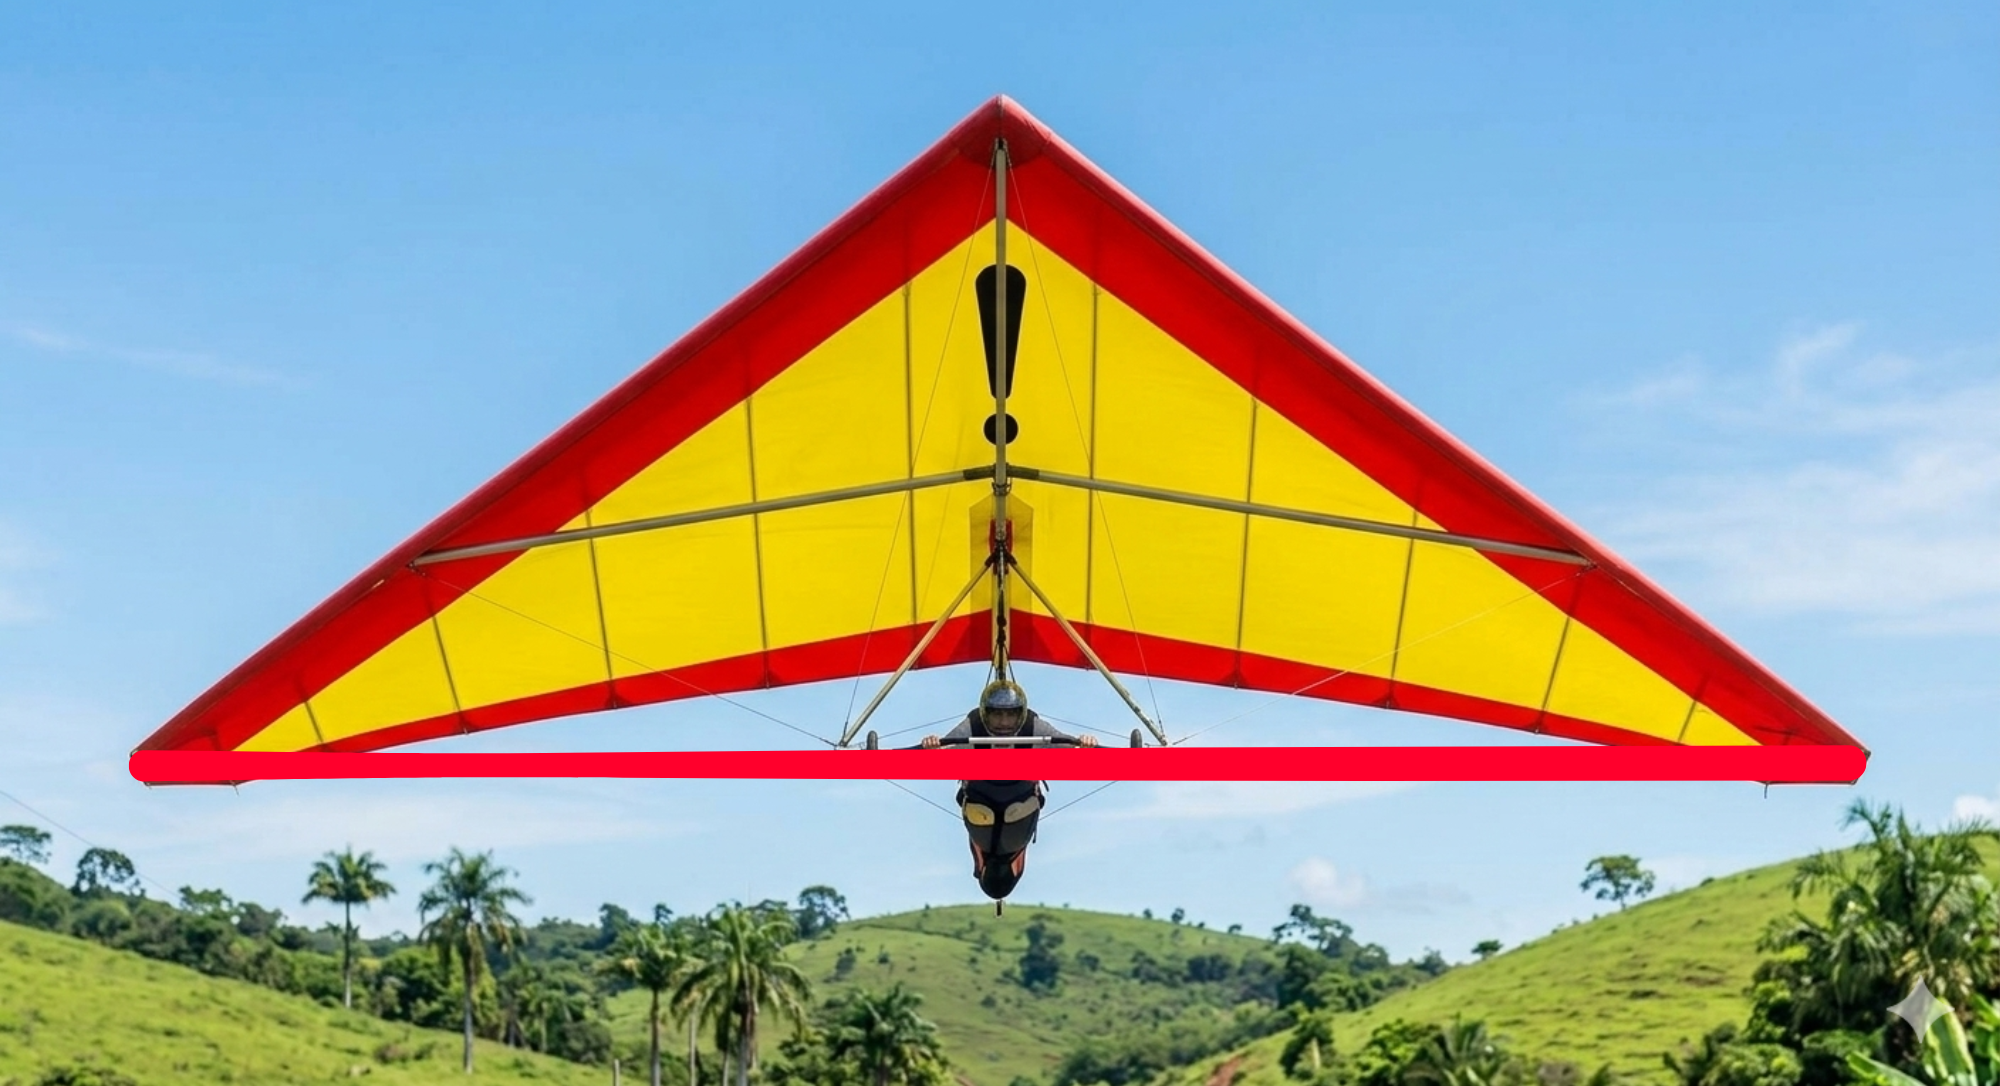
\includegraphics[width=0.5\linewidth]{figuras/6_ano/Asa Delta.png}
        \end{figure}
        Ao ver a foto, o aluno percebeu que poderia classificar esse triângulo. Qual seria a classificação dele considerando os seus ângulos?
         \begin{multicols}{4}
            \begin{enumerate}[label=\alph*)]
                \item retângulo
                \item obtusângulo
                \item acutângulo
                \item minervângulo
            \end{enumerate}
        \end{multicols}

\begin{solucoes}{1}
    \solucao
Nesta questão tem-se um triângulo gerado pela união das duas extremidades inferiores de uma asa-delta. A questão nos informou que os ângulos inferiores gerados possuem $30^\circ$, o que qualifica esse triângulo como isósceles. Como a soma dos ângulos internos de um triângulo vale $180^\circ$, teremos;
        \begin{equation*}
            x+30^\circ+30^\circ =180^\circ
        \end{equation*}
        \begin{equation*}
            x =180^\circ-60^\circ
        \end{equation*}
        \begin{equation*}
            x =120^\circ
        \end{equation*}
        Logo, como temos um ângulo obtuso, o triângulo é obtusângulo.\\
        \textbf{ALTERNATIVA B)}
\end{solucoes}
\section{Probabilidade e Estatística}

\questao{(OM$^3$SP 2026 - 1$^\circ$ fase ) Os professores de Matemática da Escola Marcelo Minervo dos Santos Pimentel, realizaram uma pesquisa com 480 pessoas. Os professores perguntava aos entrevistados qual gênero de filme eles preferiam: ação, comédia, anime, terror ou outros. Este gráfico mostra o percentual de pessoas que responderam à pesquisa.}

        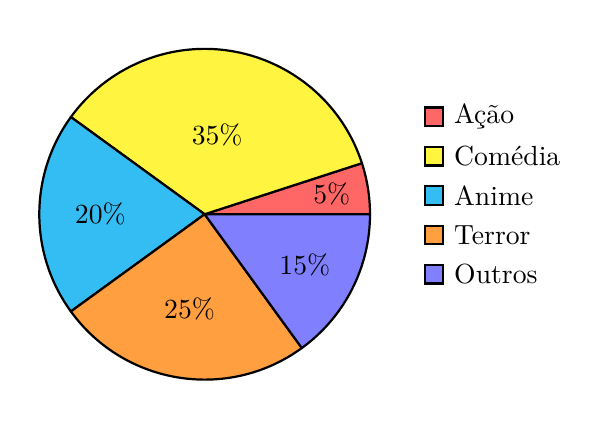
\begin{tikzpicture}[scale=.7]
            \pie[
                text=legend,
                color={red!60, yellow!75, cyan!80, orange!75, blue!50}
            ]{5/Ação, 35/Comédia, 20/Anime, 25/Terror, 15/Outros}
        \end{tikzpicture}

        Quantas pessoas responderam que preferem o gênero de filme anime?


            \begin{enumerate}[label=\alph*)]
                \item 96 pessoas
                \item 105 pessoas
                \item 90 pessoas
                \item 85 pessoas
            \end{enumerate}

\begin{solucoes}{1}
    \solucao
    Para determinar a quantidade de pessoas que preferem o gênero de filme anima, observaremos qual a sua porcentagem no gráfico e depois calcularemos quanto equivale do total de pessoas entrevistadas, assim, temos:

$\begin{WithArrows}[tikz={>=stealth, text width = 6cm, draw=black!70, text=black!70}, interline=2mm]
    Anime =& 20\%\, de\, 480  \Arrow[rl]{Transformando em um produto} \\ 
    Anime =& \dfrac{20}{100} \times 480   \\
    Anime =& \dfrac{\cancel{20}}{\cancel{100}} \times 480 
    \Arrow[ll]{Simplificando a fração por 20, temos}\\
    Anime =& \dfrac{480}{4} \\
    Anime =& 96
\end{WithArrows}$

Sendo assim, a quantidade de pessoas que preferem o gênero de filme Anime é 96

 \textbf{ALTERNATIVA D}

\end{solucoes}

\questao{Para escolher 1 entre 4 estudantes para ser presidente do grêmio da Escola Marcelo Pimentel, o coordenador Jefferson estabeleceu como critério a maior média obtida com as notas dadas \textbf{à prova escrita}, \textbf{à entrevista} e a \textbf{apresentação de ideias}. Analise as notas obtidas pelos estudantes e descubra qual o estudante escolhido.}

        \begin{figure}[H]
        \centering
            \begin{minipage}{.33\linewidth}
                \begin{tabular}{|p{2.5cm}|}
                    \hline
                    \multicolumn{1}{|c|}{ESTUDANTE 1}\\
                    \hline
                    Prova: 8 \par
                    Entrevista: 7 \par 
                    Ideias: 6
                    \\
                    \hline
                    
                \end{tabular}
            \end{minipage}
            \begin{minipage}{.33\linewidth}
                \begin{tabular}{|p{2.5cm}|}
                    \hline
                    \multicolumn{1}{|c|}{ESTUDANTE 2}\\
                    \hline
                    Prova: 8 \par
                    Entrevista: 8 \par 
                    Ideias: 7
                    \\
                    \hline
                    
                \end{tabular}
            \end{minipage}
            
        \end{figure}

\vspace*{-15pt}
        \begin{figure}[H]
            \centering
            \begin{minipage}{.33\linewidth}
                \begin{tabular}{|p{2.5cm}|}
                    \hline
                    \multicolumn{1}{|c|}{ESTUDANTE 3}\\
                    \hline
                    Prova: 7 \par
                    Entrevista: 6 \par 
                    Ideias: 7
                    \\
                    \hline
                    
                \end{tabular}
            \end{minipage}
            \begin{minipage}{.33\linewidth}
                \begin{tabular}{|p{2.5cm}|}
                    \hline
                    \multicolumn{1}{|c|}{ESTUDANTE 4}\\
                    \hline
                    Prova: 8 \par
                    Entrevista: 9 \par 
                    Ideias: 5
                    \\
                    \hline
                    
                \end{tabular}
            \end{minipage}
           
        \end{figure}

        \begin{multicols}{2}
            \begin{enumerate}[label=\alph*)]
                \item ESTUDANTE 1
                \item ESTUDANTE 2
                \item ESTUDANTE 3
                \item ESTUDANTE 4
            \end{enumerate}
        \end{multicols}

\begin{solucoes}{1}
\solucao

Para descobrir qual estudante foi escolhido, é preciso calcular a média de cada um dos estudantes.

\begin{multicols}{2}
    Para o estudante 1, temos:

$\begin{WithArrows}[tikz={>=stealth, text width= 6cm, draw=black!70, text=black!70}, interline=2mm]
   M &= \dfrac{8+7+6}{3} \\
   M &= \dfrac{21}{3} \\
   M &= 7
\end{WithArrows}$

Média igual a 7.

Para o estudante 2, temos:

$\begin{WithArrows}[tikz={>=stealth, text width = 6cm, draw=black!70, text=black!70}, interline=2mm]
   M &= \dfrac{8+8+7}{3}\\
   M &= \dfrac{23}{3} \Arrow[ll]{Calculando o resultado da fração, temos aproximadamente}\\
   M &= 7,6
\end{WithArrows}$

Média igual a 7,6.

Para o estudante 3, temos:

$\begin{WithArrows}[tikz={>=stealth, text width = 6cm, draw=black!70, text=black!70}, interline=2mm]
    M &= \dfrac{7+6+7}{3} \\
    M &= \dfrac{20}{3} \Arrow[ll]{Calculando o resultado da fração, temos aproximadamente}\\
    M &= 6,6
\end{WithArrows}$

Média igual a 6,6.

Para o estudante 4, temos:

$\begin{WithArrows}[tikz={>=stealth, text width = 6cm, draw=black!70, text=black!70}, interline=2mm]
    M &= \dfrac{8+9+5}{3} \\
    M &= \dfrac{22}{3} \Arrow[ll]{Calculando o resultado da fração, temos aproximadamente}\\
    M &= 7,3
\end{WithArrows}$

Média igual a 7,3.
\end{multicols}

Fazendo a comparação das médias obtidas por cada estudante, temos:

estudante 2 $>$ estudante 4 $>$ estudante 1 $>$ estudante 3.

Assim, o escolhido foi o \textbf{estudante 2}

\textbf{ALTERNATIVA B}
    
\end{solucoes}
\section{Grandezas e Medidas}

\questao{Primeira questão}



% Questões do 7° ano

\chapter{7$^{\circ}$ Ano}

\begin{caixainfo}

\textbf{Matemática — 7$^{\circ}$ ano}

Neste capítulo estão reunidas questões destinadas ao 7$^{\circ}$ ano do Ensino Fundamental, organizadas de acordo com as Unidades Temáticas da BNCC.

\end{caixainfo}

\vspace{1cm}

\section*{Unidades Temáticas}

\begin{center}

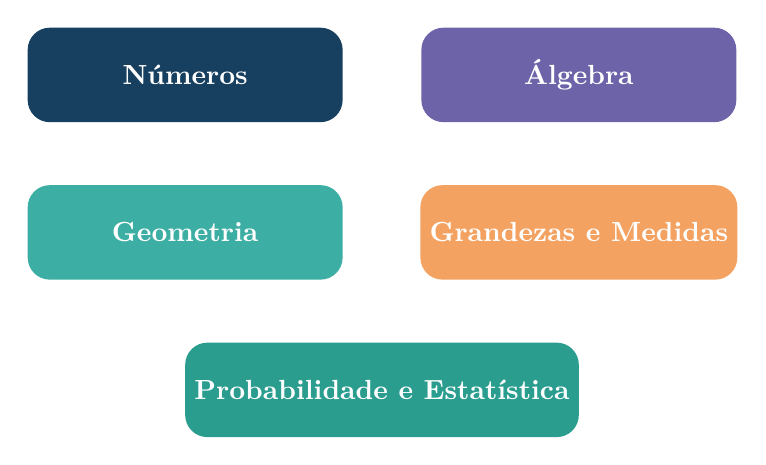
\begin{tikzpicture}

\node[
    rounded corners=8pt,
    fill=AzulPrincipal,
    text=white,
    minimum width=4cm,
    minimum height=1.2cm
] (n) at (0,0) {\textbf{Números}};

\node[
    rounded corners=8pt,
    fill=Roxo,
    text=white,
    minimum width=4cm,
    minimum height=1.2cm
] (a) at (5,0) {\textbf{Álgebra}};

\node[
    rounded corners=8pt,
    fill=Turquesa,
    text=white,
    minimum width=4cm,
    minimum height=1.2cm
] (g) at (0,-2) {\textbf{Geometria}};

\node[
    rounded corners=8pt,
    fill=Laranja,
    text=white,
    minimum width=4cm,
    minimum height=1.2cm
] (m) at (5,-2) {\textbf{Grandezas e Medidas}};

\node[
    rounded corners=8pt,
    fill=Verde,
    text=white,
    minimum width=4cm,
    minimum height=1.2cm
] (p) at (2.5,-4) {\textbf{Probabilidade e Estatística}};

\end{tikzpicture}

\end{center}

\clearpage


\section{Números}

\questao{Primeira questão}


\section{Álgebra}

\questao{(Elaboração própria) Escreva a expressão algébrica que corresponde à sentença dada. Depois, determine o valor numérico dela para x = 12.}

O dobro de um número mais um terço desse mesmo número.

\begin{multicols}{4}
    \begin{enumerate}[label=\alph*) ]
        \item 24
        \item 28
        \item 27
        \item 34
    \end{enumerate}
\end{multicols}

% Caso a questão tenha mais de uma solução, alterar o valor da segunda chaves, que se refere ao valor para a quantidade de soluções que a questão terá.
% e insira o comando \solucao para uma nova resolução do item.
\begin{solucoes}{1}
\solucao

    Primeiro, transformamos a linguagem usual em linguagem matemática, assim, temos a seguinte expressão algébrica:

    \begin{equation*}
        2x + \cfrac{1}{3}\times x
    \end{equation*}

    Substituindo o valor dado na questão, temos:
    
    \begin{equation*}
        2 \times 12 + \cfrac{1}{3} \times 12 = 24 + \cfrac{12}{3} = 24 + 4 = 28
    \end{equation*}

    Então, o valor numérico da expressão algébrica é 28. \\
    \textbf{ALTERNATIVA B)}
\end{solucoes}

\questao{(OM$^3$SP 2026 - 1ª Fase) Em um dia na E.M.M.M.S.P. a diretora Sheyla propôs um desafio matemático. Aquele que acertasse seria dispensado de suas duas últimas aulas. Ela propôs o seguinte desafio: \textquotedblleft Vinte rapaduras custam $R\$ \ 60,00$ a mais do que cinco rapaduras. Qual o valor de uma rapadura?\textquotedblright\, Pensando na dispensa das duas últimas aulas, qual é o valor de uma rapadura?}
        \begin{multicols}{4}
            \begin{enumerate}[label=\alph*)]
                \item $R\$ \ 3,50$
                \item $R\$ \ 4,00$
                \item $R\$ \ 4,50$
                \item $R\$ \ 5,00$
            \end{enumerate}
        \end{multicols}

\begin{solucoes}{2}
    \solucao
    Temos aqui um problema clássico da álgebra e para resolvermos utilizaremos como método de solução uma equação do  primeiro grau. A diretora Sheyla propôs que vinte rapaduras custam $R\$ \ 60,00$ a
mais do que cinco rapaduras. Não sabemos o valor de cada rapadura, assim chame o número de rapaduras de $x$ e assim teremos:
\begin{equation*}
20x=60+5x
\end{equation*}
\begin{equation*}
20x-5x=60
\end{equation*}\begin{equation*}
15x=60
\end{equation*}
\begin{equation*}
x=\frac{60}{15}
\end{equation*}
\begin{equation*}
x=4.
\end{equation*}
Logo, o valor de cada rapadura é $R\$ \ 4,00$.\\
\textbf{ALTERNATIVA B)}

\solucao
Muitas vezes existe uma dificuldade de observação frente aos problemas algébricos. Mas, é possível resolvê-lo sem necessariamente saber montar uma equação. O enunciado nos diz que vinte rapaduras custam o mesmo que cinco rapaduras mais $R\$ \ 60,00$. Com isso, podemos perceber que se subtrairmos as vinte rapaduras das outras cinco, teremos a quantidade de rapaduras que valem exatamente $R\$ \ 60,00$. Logo, $20-5=15$ e assim descobrimos que $15$ rapaduras equivalem a $R\$ \ 60,00$. Para descobrir o valor de uma rapadura, é só dividir os $R\$ \ 60,00$ por $15$. Como, $\frac{60}{15}=4$, então uma rapadura vale exatamente $R \$ \ 4,00$ \\
    \textbf{ALTERNATIVA B)}
\end{solucoes}

\questao{(OM$^3$SP 2026 - 1ª Fase)Os números triangulares foram sistematizados pela escola pitagórica. Esses números são representados, com exceção do primeiro, por triângulos equiláteros (triângulos com os três lados iguais). Na imagem abaixo estão os cinco primeiros números triangulares:}
        \begin{figure}[H]
            \centering
            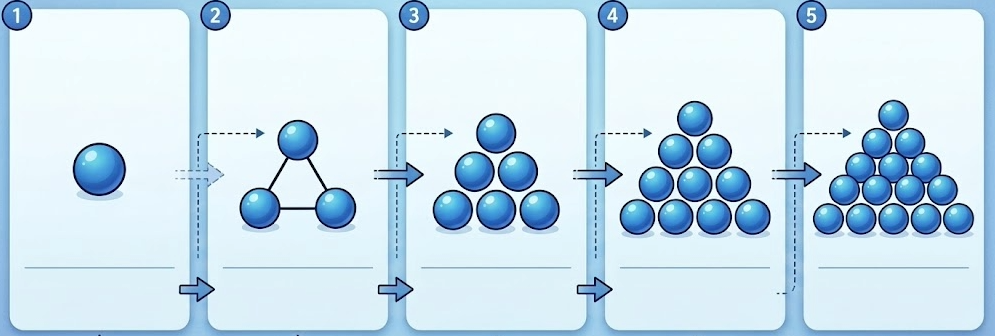
\includegraphics[width=0.9\linewidth]{figuras/7_ano/Números Triangulares.png}
        \end{figure}
        Qual o número de bolinhas no oitavo número triangular?
        \begin{multicols}{4}
            \begin{enumerate}[label=\alph*)]
                \item $21$
                \item $28$
                \item $36$
                \item $45$
            \end{enumerate}
        \end{multicols}

\begin{solucoes}{2}
    \solucao 
Os números triangulares são números interessantíssimos. Percebemos que os números triangulares estão dispostos em uma sequência numérica da seguinte forma: $T_n=\{1,3,6,10,15,...\}$. Agora, é preciso que encontremos o oitavo número triangular. Se percebermos o padrão de crescimento, veremos que do $1^\circ$ para o $2^\circ$ aumentou-se em duas unidades. Do $2^\circ$ para o $3^\circ$ aumentou-se em três unidades e assim por diante. Logo,
        \begin{equation*}
        T_6=15+6=21
        \end{equation*}
         \begin{equation*}
        T_7=21+7=28
        \end{equation*}
         \begin{equation*}
        T_8=28+8=36
        \end{equation*}
        o $8^\circ$ número triangular é o 36. \\
    \textbf{ALTERNATIVA C)}

    \solucao
    Os números triangulares são números interessantíssimos. Percebemos que os números triangulares estão dispostos em uma sequência numérica da seguinte forma: $T_n=\{1,3,6,10,15,...\}$. Agora, é preciso que encontremos o oitavo número triangular. Se percebermos o padrão de crescimento, veremos que $T_2=1+2$, $T_3=1+2+3$, $T_4=1+2+3+4$ e $T_5=1+2+3+4+5$. Sendo assim, podemos modular o termo geral da seguinte forma:
        
        \begin{equation*}
        T_n=1+2+3+4+...+(n-1)+n \\\\\\\ (1)
        \end{equation*}
        \begin{equation*}
        T_n=n+(n-1)+...+4+3+2+1 \\\\ (2)
 \end{equation*}
        
        somando $(1)$ e $(2)$:
        \begin{equation*}
        2T_n=(n+1)+(n+1)+...+(n+1)
        \end{equation*}
        \begin{equation*}
        2T_n=n\cdot(n+1)
        \end{equation*}
        \begin{equation*}
        T_n=\frac{n\cdot(n+1)}{2})
        \end{equation*}
        Logo, para determinar o oitavo número triangular substituiremos $n=8$. Com isso, 
        \begin{equation*}
            T_8=\frac{8\cdot(8+1)}{2}=\frac{8\cdot 9}{2}=\frac{72}{2}=36
        \end{equation*}
        Portanto, o $8^\circ$ número triangular é o 36. \\
    \textbf{ALTERNATIVA C)}
\end{solucoes}

\questao{(OM$^3$SP 2026 - 1ª Fase) O ring do UFC tem o formato de um octágono. O professor Samuel fez a medida dos lados do ring, mas para trabalhar os princípios algébricos, trocou o valor numérico por letras. Qual será o perímetro do ring considerando os lados apresentados na figura abaixo?}
        \begin{figure}[H]
            \centering
            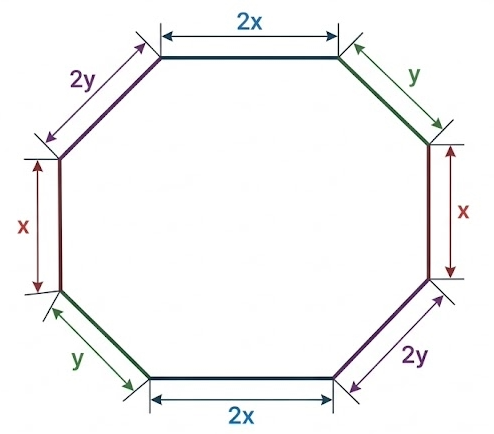
\includegraphics[width=0.5\linewidth]{figuras/7_ano/Perímetro.png}
        \end{figure}
        \begin{multicols}{4}
            \begin{enumerate}[label=\alph*)]
                \item $6x+6y$
                \item $6x+4y$
                \item $4x+6y$
                \item $4x+4y$
            \end{enumerate}
        \end{multicols}

\begin{solucoes}{1}
    \solucao
    
    Para resolver esta questão é preciso recordar a noção de perímetro. O prerímetro é a soma de todos os lados da figura e assim teremos:
        \begin{equation*}
            2P=2x+y+x+2y+2x+y+x+2y
        \end{equation*}
        e ao reduzir os termos iguais,
        \begin{equation*}
            2P=6x+6y.
        \end{equation*}
        Então, o perímetro deste ring vale 
        $6x+6y$.  \\
    \textbf{ALTERNATIVA A)}
\end{solucoes}

\questao{(OM$^3$SP 2026 - 1ª Fase)Ao ler o jornal pela manhã o coordenador Jefferson observou uma notícia intrigante:\\\\
        \textbf{No último sábado foi calculado uma preciptação de 150mm a mais do que a preciptação da sexta-feira. Além disso, no domingo foi calculado uma preciptação de 30mm a menos que na sexta-feira}. \\\\ O coordenador Jefferson lembrou que no sábado choveu 200mm. Sendo assim, quanto choveu no domingo?}
        \begin{multicols}{4}
            \begin{enumerate}[label=\alph*)]
                \item $50mm$
                \item $40mm$
                \item $30mm$
                \item $20mm$
            \end{enumerate}
        \end{multicols}
\begin{solucoes}{2}
\solucao
    Olhando para a manchete que o coordenador Jefferson leu, podemos ver que, (considere sexta como $x$, sábado como $y$ e domingo como $z$)
        \begin{equation*}
            y=x+150 \ (1)
        \end{equation*}
        \begin{equation*}
              z=x-30. \ (2)
        \end{equation*}
        Jefferson sabia que a precipitação de sábado foi de $200mm$, ou seja, $y=200$. Substituindo esta informação em $(1)$,
        \begin{equation*}
            200=x+150 \Longrightarrow x=50mm. \ (3)
        \end{equation*}
        Assim, por $(3)$, a precipitação de sexta foi de $50mm$. Por fim, substituindo $
        (3)$ em $(2)$,
        \begin{equation*}
            z=50-30=20mm. \ (4)
        \end{equation*}
Assim, por $(4)$, no domingo a precipitação foi de $20mm$. \\
    \textbf{ALTERNATIVA D)}

\solucao

Muitos discentes possuem dificuldades coma linguagem algébrica e podemos resolver este problema sem necessariamente precisarmos montar as expressões algébricas. Sabemos que no sábado choveu $200mm$ e que no sábado choveu $150mm$ a mais que na sexta, então na sexta choveu $200m-150mm=50mm$. Sabemos também que no domingo choveu $30mm$ a menos que na sexta, assim $50mm30mm=20mm$. Logo,no domingo, a preciptação foi de $20mm$.   \\
    \textbf{ALTERNATIVA D)}

\end{solucoes}

\questao{(OM$^3$SP 2026 - 1ª Fase)O professor Jadiel gosta muito de comer salgadinho de padaria. Todavia, por comer muito, teve uma orientação nutricional de diminuir a quantidade de salgadinho ingerido até não comer mais nenhum. No primeiro dia ele comeu 45 salgadinhos, no segundo dia ele comeu 44 salgadinhos, no terceiro dia ele comeu 42 salgadinhos, no quarto dia ele comeu 39 salgadinhos e assim por diante. Em qual dia ele deixou de comer os salgadinhos?}
         \begin{multicols}{4}
            \begin{enumerate}[label=\alph*)]
                \item $6^\circ$  dia
                \item $8^\circ$ dia
                \item $10^\circ$  dia
                \item $12^\circ$  dia
            \end{enumerate}
        \end{multicols}

\begin{solucoes}{2}
\solucao
A questão nos deu os seguintes números: $S_n=\{45,44,42,39,...\}$. Agora, é preciso que encontremos o dia em que o professor Jadiel parou de comer salgadinhos. Se percebermos o padrão de decrescimento, veremos que do $1^\circ$ para o $2^\circ$ diminuiu-se em uma unidade. Do $2^\circ$ para o $3^\circ$ diminuiu-se em duas unidades e assim por diante. Logo,
 \begin{equation*}
     S_5=39-4=35
 \end{equation*}
  \begin{equation*}
     S_6=35-5=30
 \end{equation*}
 \begin{equation*}
     S_7=30-6=24
 \end{equation*}
  \begin{equation*}
     S_8=24-7=17
 \end{equation*}
 \begin{equation*}
     S_9=17-8=9
 \end{equation*}
  \begin{equation*}
     S_{10}=9-9=0
 \end{equation*}
 Logo, no décimo dia o professor Jadiel parará de comer salgadinhos.   \\
    \textbf{ALTERNATIVA C)}

\solucao
Podemos pensar também algebricamente. Tem-se aí um princípio de sequência de termos onde o próximo termo é sempre o anterior subtraido de um mesmo número, no caso o número $1$. Queremos determinar o tempo $n$ para $a_n=o$. Agora, é preciso que encontremos o oitavo número triangular. Se percebermos o padrão de crescimento, veremos que $a_2=45-1$, $a_3=45-1-2$, $a_4=45-1-2-3$ e $a_5=45-1-2-3-4$. Sendo assim, podemos modular o termo geral da seguinte forma:
  
        \begin{equation*}
        a_n=45-1-2-3-...-(n-1) \ 
        \end{equation*}
        \begin{equation*}
        a_n=45-(1+2+3+4+5+...+n-1)
 \end{equation*}
 \begin{equation*}
     a_n= 45-\frac{(n-1)*n}{2}
 \end{equation*}
        
Logo, como queremos mostrar o valor de $n$ para que $a_n$ seja $0$, faremos
\begin{equation*}
    0=45-\frac{(n-1)*n}{2}
\end{equation*}
\begin{equation*}
    \frac{(n-1)*n}{2}=45
\end{equation*}
\begin{equation*}
    (n-1)*n=90
\end{equation*}
\begin{equation*}
    (n-1)*n=9*10
\end{equation*}
\begin{equation*}
    (n-1)*n=(10-1)*10
\end{equation*}

Sendo assim, $n=10$. Logo, no décimo dia o professor Jadiel parará de comer salgadinhos. 
\\
\textbf{ALTERNATIVA C)}
\end{solucoes}

\questao{(OAM 2025 - NÍVEL 1) Os múltiplos de 3 foram escritos seguindo o padrão da figura ao lado. Sabe-se que Clarisse continuou escrevendo até a décima linha e depois somou o primeiro com o último número que aparecem nessa linha. Qual o valor encontrado por Clarisse?}
\begin{figure}[H]
    \centering
    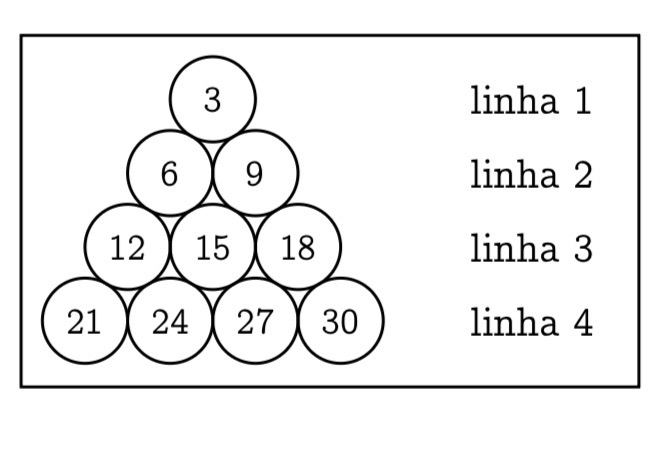
\includegraphics[width=0.5\linewidth]{figuras/7_ano/IMG_0943.jpeg}
    \label{fig:placeholder}
\end{figure}

\begin{solucoes}{2}
    \solucao
    Vemos na imagem abaixo um padrão claro, os números são formados pelos múltiplos de três em sua ordem. A imagem é bem clara na sequência de termos e percebemos que cada bola está na sequência de múltiplos de $3$. Cada linha tem exatamente o mesmo número de bolas do número da linha. A linha quatro possui $3\cdot 7=21$, $3\cdot8=24$, $3\cdot 9=27$ e $3\cdot 10=30$. Podemos determinar a sequência a partir da quinta linha e irmos até a décima:
\\\\
    $i)$ Linha 5
\\\\
    $3\cdot 11=33$, $3\cdot 12=36$, $3\cdot 13=39$, $3\cdot 14=42$, $3\cdot 15=45$.
\\\\
    $ii)$ Linha 6
\\\\
    $3\cdot 16=48$, $3\cdot 17=51$, $3\cdot 18=54$, $3\cdot 19=57$, $3\cdot 20=60$ e $3\cdot 21=63$.
\\\\
    $iii)$ Linha 7
\\\\
    $3\cdot 22=66$, $3\cdot 23=69$, $3\cdot 24=72$, $3\cdot 25=75$, $3\cdot 26=78$, $3\cdot 27=81$ e $3\cdot 28=84$.
\\\\
    $iv)$ Linha 8
\\\\
    $3\cdot 29=87$, $3\cdot 30=90$, $3\cdot 31=93$, $3\cdot 32=96$, $3\cdot 33=99$, $3\cdot 34=102$, $3\cdot 35=105$ e $3\cdot36=108$.
\\\\
    $v)$ Linha 9
\\\
       $3\cdot 37=111$, $3\cdot 38=114$, $3\cdot 39=117$, $3\cdot 40=120$, $3\cdot 41=123$, $3\cdot 42=126$, $3\cdot 43=129$, $3\cdot 44=132$ e $3\cdot45=135$.
\\\\
    $vi)$ Linha 10
\\\\
    $3\cdot 46=138$, $3\cdot 47=141$, $3\cdot 48=144$, $3\cdot 49=147$, $3\cdot 50=150$, $3\cdot 51=153$, $3\cdot 52=156$, $3\cdot 53=159$, $3\cdot 54=162$ e $3\cdot 55=165$.
\\\\
Queremos a soma do primeiro e do último da linha 10, assim $138+165=303$.

\solucao
Se pensarmos aqui temos uma sequência de termos que possui uma razão constante (enrolando um pouco para não utilizar o termo progressão aritmética). Logo, se pensarmos em termo geral, temos que todos os elementos são múltiplos de 3. Logo $a_n=3\cdot n$. Para descobrir o último termo podemos pensar da seguinte maneira apenas somando as linhas $1+2+3+4+5+6+7+8+9+10=55$ e teríamos que o último termo é $a_{55}=3\cdot 55=165$ e o primeiro termo da linha seria o $a_{46}=3\cdot 46=138$. Assim, $138+165=303$.

\end{solucoes}

\section{Geometria}

\questao{(OM$^3$SP 2026 - 2ª Fase) Tales de Mileto (c. 624 – 548 a.C.), foi um comerciante, matemático e astrônomo nascido na colônia jônica de Mileto (atual Turquia), é amplamente considerado por Aristóteles e pela tradição historiográfica como o primeiro filósofo do Ocidente e um dos Sete Sábios da Grécia Antiga. Uma proposição atribuída a ele é a Lei Angular de Tales que diz,} 

                \begin{Teorema}{Lei Angular de Tales}
                     Dado um triângulo de vértices $A$, $B$ e
                     $C$, de ângulos internos $\widehat A$, $\widehat B$ e $\widehat C$, a soma dos ângulos internos deste triângulo equivale a $180\text{°}$.
                \end{Teorema}
                \begin{figure}[H]
                    \centering
                    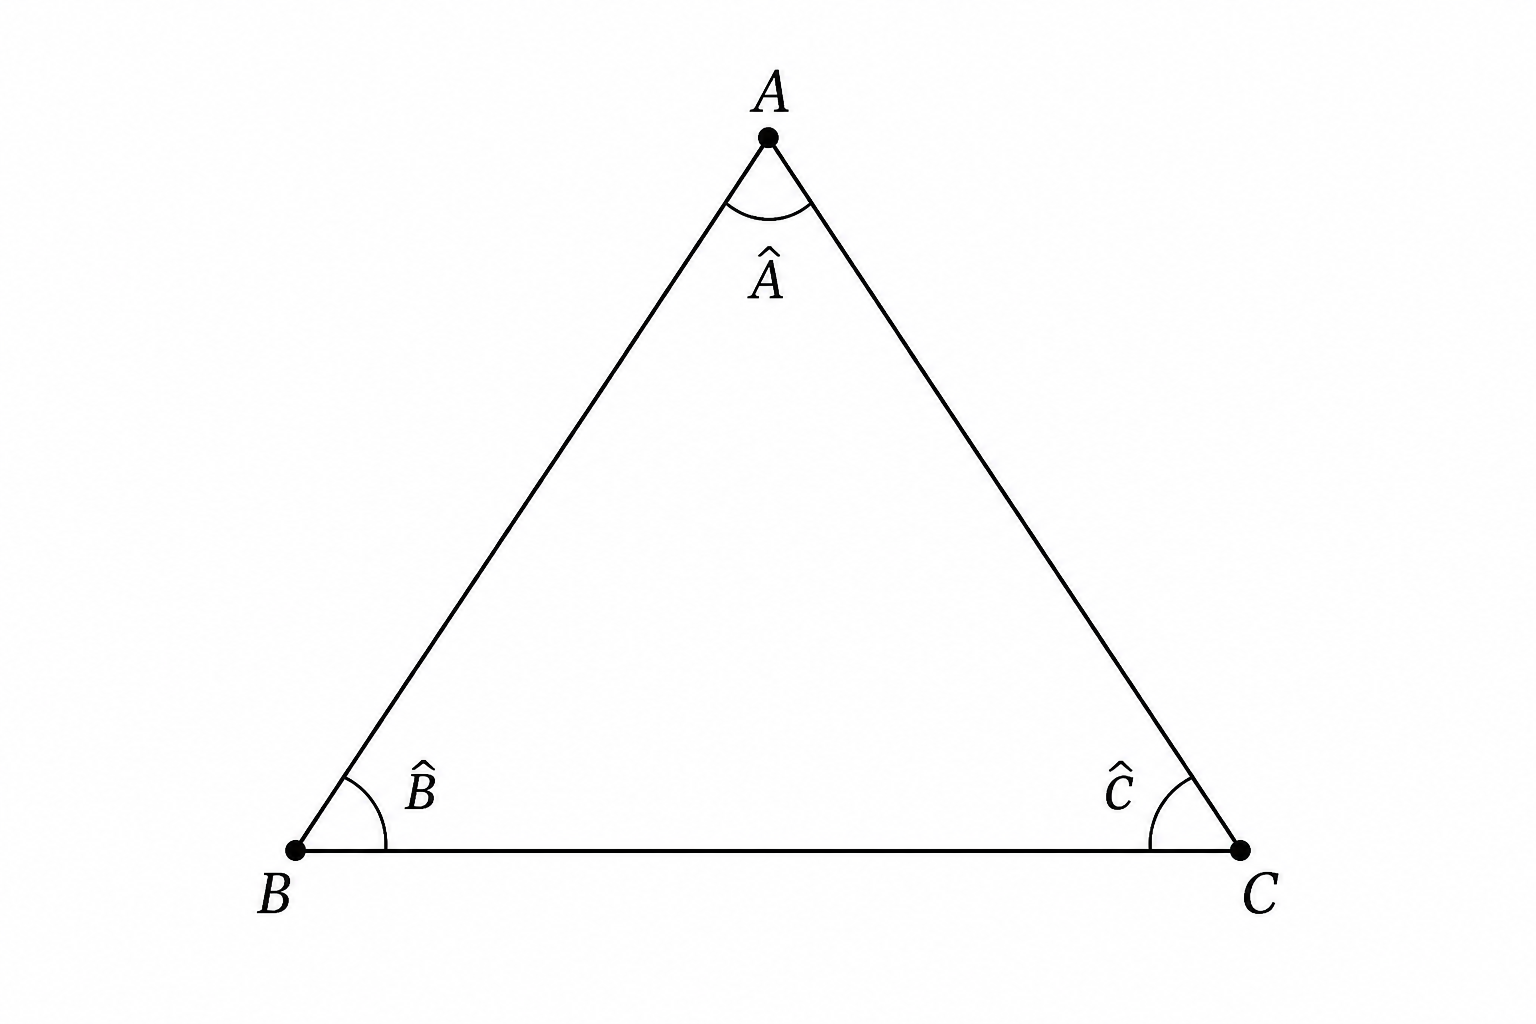
\includegraphics[width=0.45\linewidth]{figuras/7_ano/Max_a_Marque_também_os_vér.png}
                \end{figure}
           \begin{enumerate}[label=\alph*)]  
           \item Assumindo que o Teorema 1 é válido, qual será o valor do ângulo interno desconhecido de um triângulo, sabendo que os outros dois valem $25\text{°}$ e $120\text{°}$?
           
            \item Com base no que foi dito no Teorema 1, demostre que o que foi afirmado é possível.           
\item Em consequência ao item b, é possível determinar um teorema muito importante,
\begin{Teorema}{Teorema do Ângulo Externo}
     Dado um triângulo de vértices $A$, $B$ e $C$, de ângulos internos $\widehat A$, $\widehat B$ e $\widehat C$, o ângulo externo ao ângulo interno $\widehat C$ equivale a soma dos ângulos $\widehat A$ e $\widehat B$ .
\end{Teorema}
Com base no que foi dito no Teorema 2, demostre que o que foi afirmado é possível.
\end{enumerate}
% Caso a questão tenha mais de uma solução, alterar o valor da segunda chaves, que se refere ao valor para a quantidade de soluções que a questão terá.
% e insira o comando \solucao para uma nova resolução do item.

\begin{solucoes}{1}
    \solucao
\textbf{Item a)}

    Em primeiro lugar, não se deve fazer nada mais do que apenas utilizar o Teorema 1 proposto. Assim, assumindo que ele é válido e tendo dois ângulos determinados, no valor de $25\text{°}$ e $120\text{°}$,
    
\begin{equation*}
    \widehat A+ \widehat B+ \widehat C=180\text{°}
\end{equation*}
\begin{equation*}
    25\text{°}+120\text{°}+\widehat C=180\text{°}
\end{equation*}
\begin{equation*}
    145\text{°}+\widehat C=180\text{°}
\end{equation*}
\begin{equation*}
     \widehat C=180\text{°}-145\text{°}
\end{equation*}
\begin{equation*}
    \fbox{$\widehat C=35\text{°}$}
\end{equation*}

Logo, considerando que o Teorema 1 é válido, o valor do ângulo interno desconhecido será $35\text{°}$.
\end{solucoes}

% Caso a questão tenha mais de uma solução, alterar o valor da segunda chaves, que se refere ao valor para a quantidade de soluções que a questão terá.
% e insira o comando \solucao para uma nova resolução do item.
\begin{solucoes}{1}

\solucao

\textbf{Item b)}

Após mostrar a usualidade do Teorema 1 no \textbf{item a)}, uma pergunta deve surgir: Será que este Teorema é sempre válido? Dentro da geometria euclidiana, ele será sempre válido, todavia é preciso que se prove esta verdade. Sendo assim, considere um triângulo de vértices  $A, B \ \text{e} \ C$, se traçarmos uma reta tangente ao vértice $A$ e prolongarmos as retas que passam pelos vértices $A, B \ \text{e} \ C$, teremos

\begin{figure}[H]
    \centering
    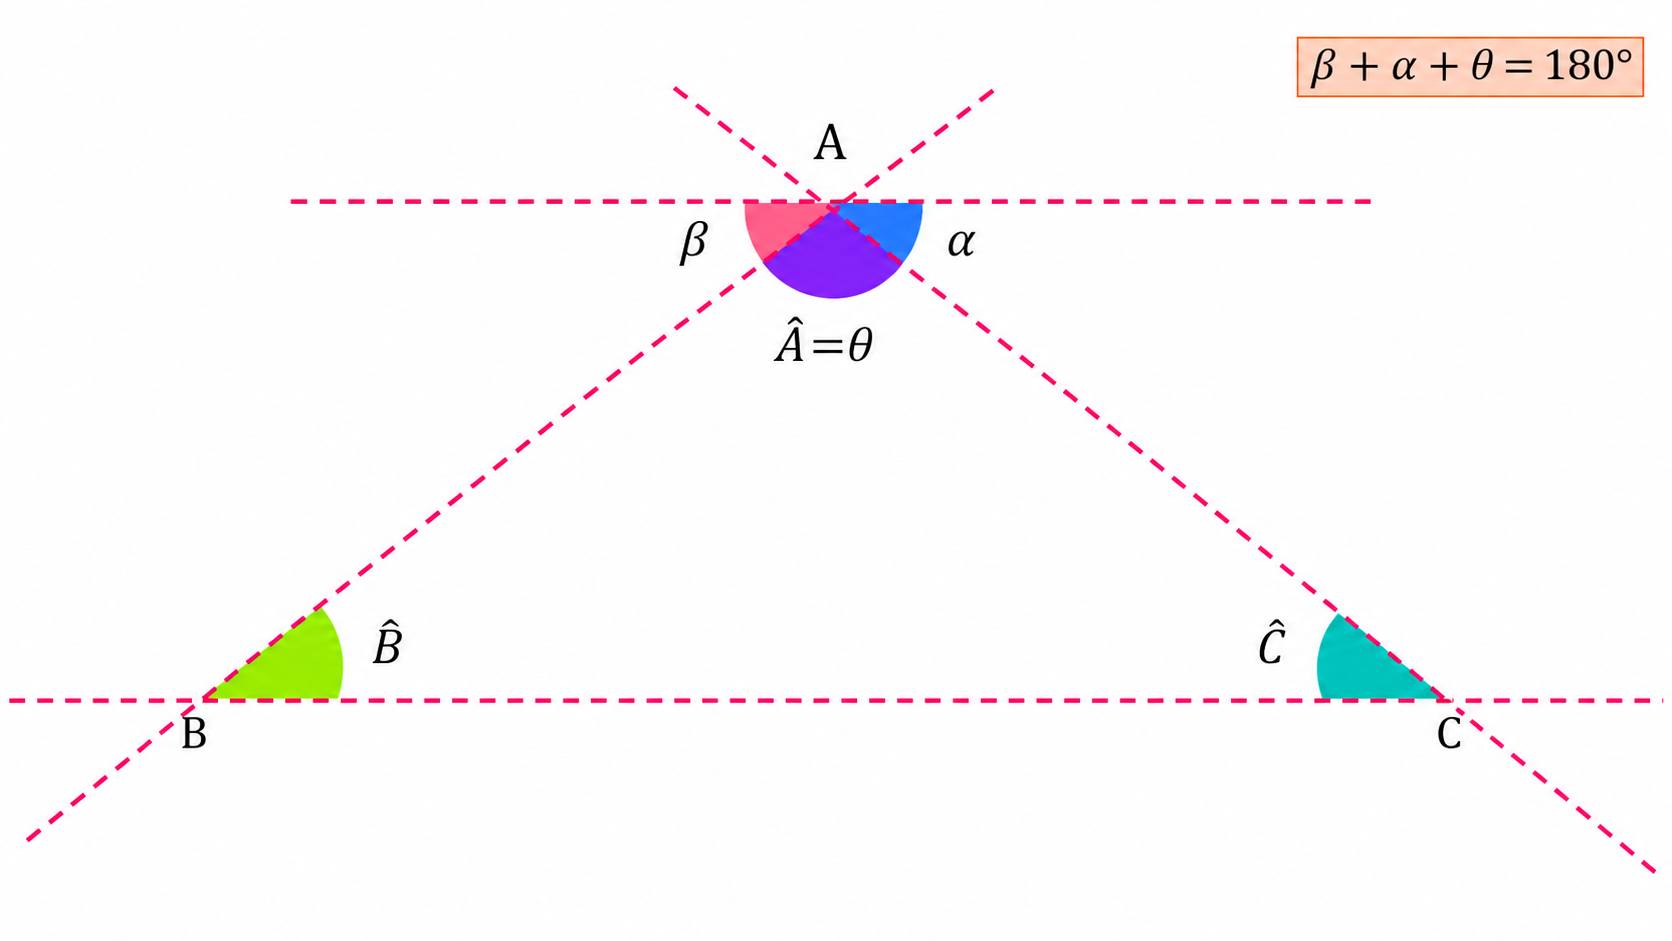
\includegraphics[width=0.7\linewidth]{figuras/7_ano/Max_a_gere_esta_imagem_em_.png}
\end{figure}

Perceba, no triângulo acima, que os ângulos $\alpha$, $\beta$ e $\widehat A \equiv \theta$ somados totalizam $180\text{°}$. Se observarmos bem, temos que o ângulo $\beta$ é correspondente ao ângulo que está oposto pelo vértice ao ângulo $\widehat B$ e o ângulo $\alpha$ é correspondente ao ângulo que está oposto pelo vértice ao ângulo $\widehat C$, como a imagem a seguir nos mostra,
\begin{figure}[H]
    \centering
    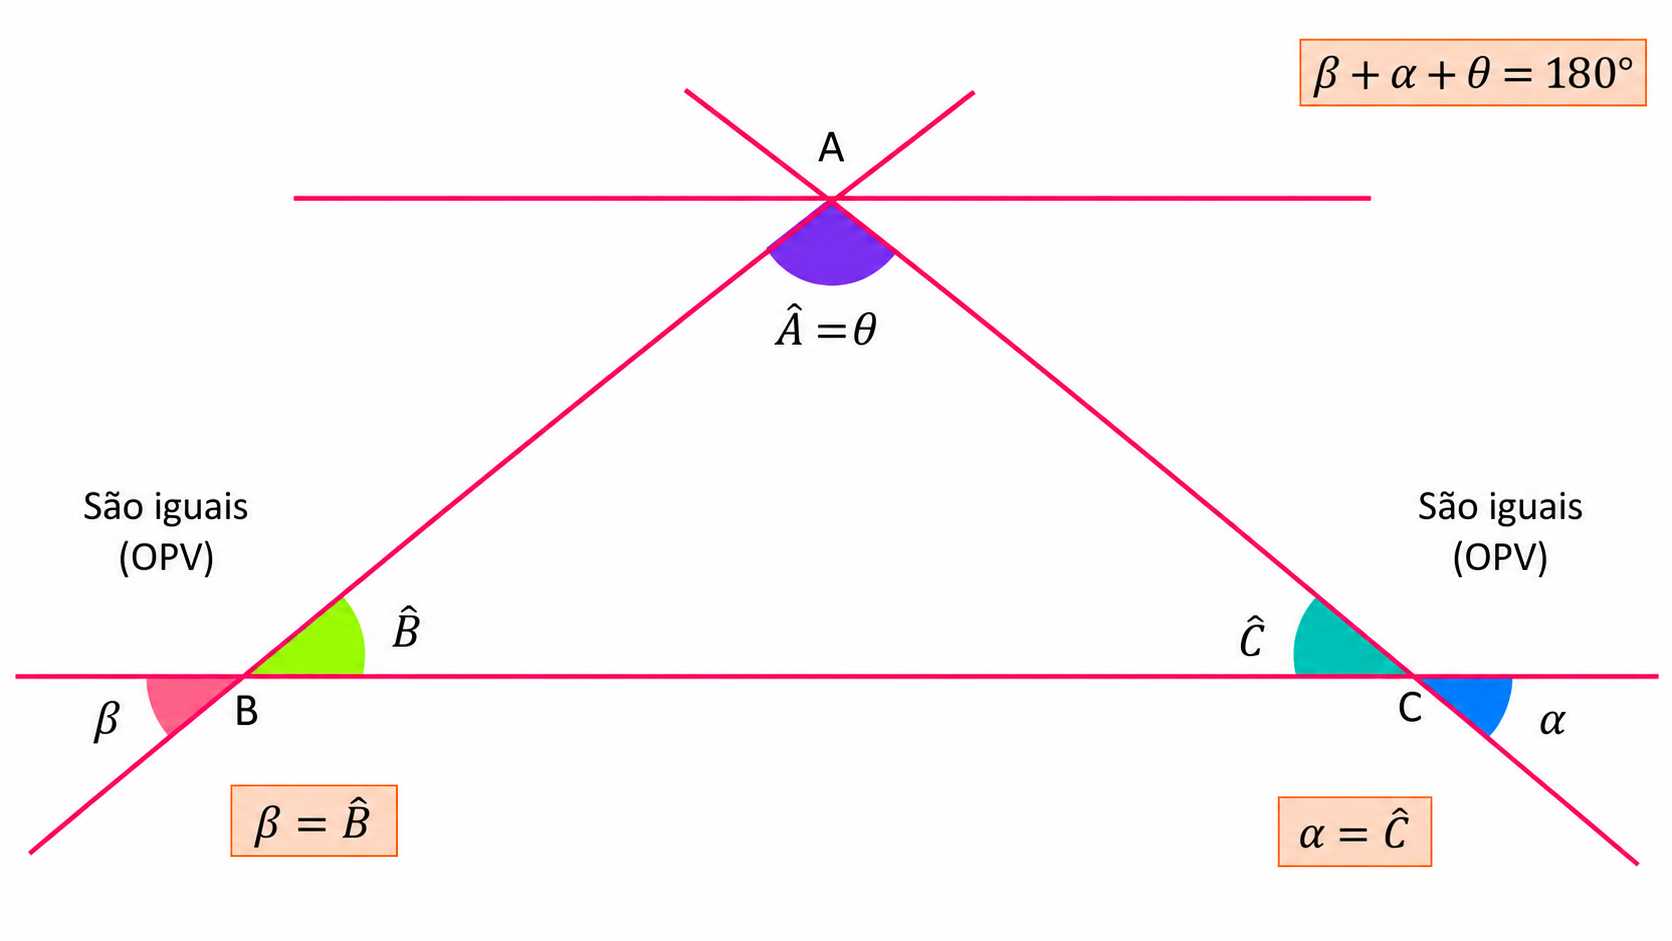
\includegraphics[width=0.7\linewidth]{figuras/7_ano/Max_a_gere_esta_imagem_em_ (1).png}
    \label{fig:placeholder}
\end{figure}
    Por definição, dois ângulos que são opostos pelo vértice são congruentes. Logo, $\beta \equiv \widehat B$ e $\alpha \equiv \widehat C$. Com isso, chegamos à conclusão do item b, pois 
    \begin{equation*}
        \alpha+\beta+\theta=180^°
    \end{equation*}
e como $\alpha \equiv \widehat C$, $\widehat A \equiv \theta$ e $\beta \equiv \widehat B$, concluímos que
    \begin{equation*}
        \widehat A+\widehat B+\widehat C=180^°
    \end{equation*} 

\solucao

\textbf{Item c)} 

Após mostrar a lei angular de Tales, o Teorema do ângulo Externo se torna quase que uma consequência. Observe a figura a seguir,
\begin{figure}[H]
    \centering
    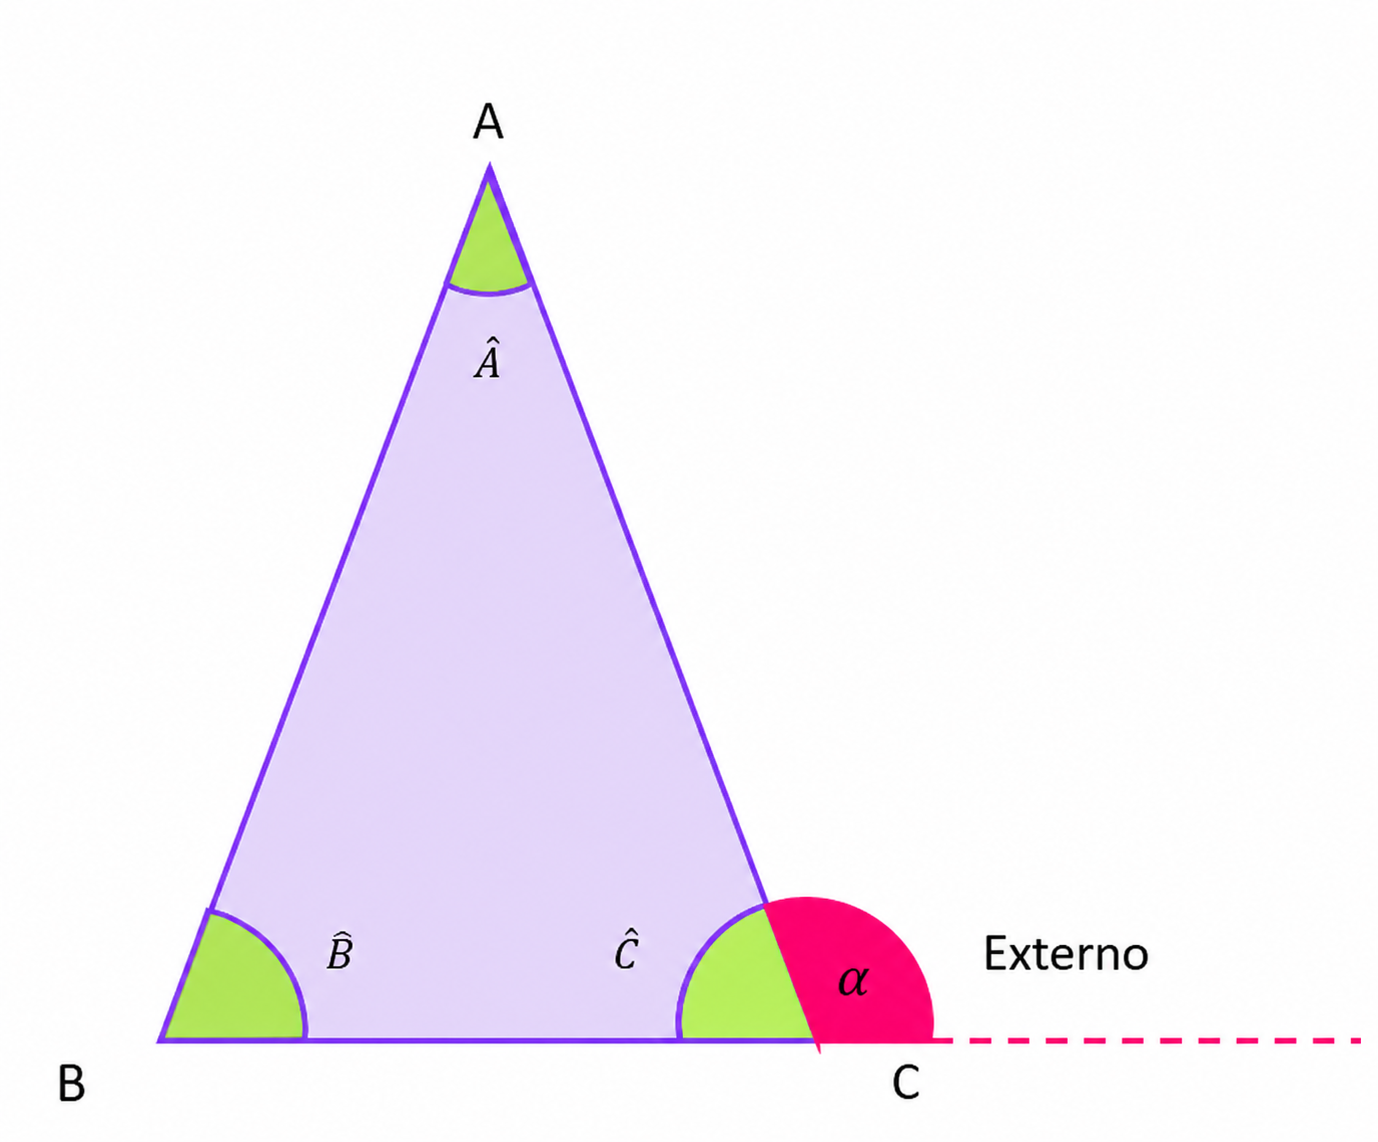
\includegraphics[width=0.45\linewidth]{figuras/7_ano/Max_a_não_mude_nada_da_fot.png}
    \label{fig:placeholder}
\end{figure}
Duas coisas devem saltar aos nossos olhos. Em primeiro lugar, pelo item b) sabemos que $ \widehat A+\widehat B+\widehat C=180^\textit{°}$. Em segundo, e último lugar, sabemos que $\widehat C+\alpha=180\textit{°}$, pois os dois são ângulos suplementares. Após essas duas definições só nos resta utilizarmos as ferramentas aritméticas para resolver este enigma e assim,
\begin{equation*}
  \begin{cases}
    \widehat A+\widehat B+\widehat C=180^° \\
    \widehat C+\alpha=180\textit{°}
  \end{cases}
\end{equation*}
Se pegarmos a primeira equação e subtrai-la pela segunda teremos que

\begin{equation*}
    \widehat A+\widehat B-\alpha=0 
\end{equation*}
\begin{equation*}
        \widehat A+\widehat B=\alpha
\end{equation*}
Logo, o ângulo externo ao ângulo $\widehat C$ equivale a soma dos ângulos internos $\widehat A \ e \ \widehat B$.
\end{solucoes}

\questao{(OM$^3$SP 2026 - 1$^\circ$ fase) Um jogo de Tangram foi montado a partir de sete peças recortadas de um quadriculado, no qual cada quadradinho possui lado de 1 cm, conforme ilustrado na figura a seguir.}

        \begin{center}
            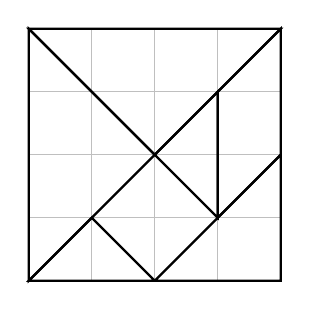
\begin{tikzpicture}[scale=.8]
                \draw[step=1cm, very thin, gray!50](0,0) grid (4,4);

                \draw[thick](0,0)--(2,2)--(0,4) -- cycle;
                \draw[thick](2,2)--(4,4)--(0,4)--cycle;
                \draw[thick](0,0)--(1,1)--(2,0)-- cycle;
                \draw[thick](2,2)--(3,1)--(3,3)-- cycle;
                \draw[thick](2,0)--(4,0)--(4,2)-- cycle;
                \draw[thick](3,1)--(4,2)--(4,4)--(3,3)--cycle;
                
            \end{tikzpicture}
        \end{center}

         A figura a seguir foi montada com 5 dessas peças sem sobreposição. Qual é a área dessa figura?

        \begin{figure}[H]
            \begin{minipage}{.34\linewidth}
                \begin{enumerate}[label=\alph*)]
                    \item 10 $cm^2$
                    \item 12 $cm^2$
                    \item 14 $cm^2$
                    \item 16 $cm^2$
                \end{enumerate}
            \end{minipage}
            \begin{minipage}{.65\linewidth}
                
\begin{tikzpicture}[scale=.8]
                    \fill[color=black!50, thick, rotate around={-45:(1,1)}](0,0)--(2,0)--(1,1)--cycle;
                    \fill[color=black!50, thick, rotate around={45:(1,1)}](0,0)--(2,0)--(1,1)--cycle;
                    \fill[color=black!50, thick](2.4142,1)rectangle(3.8284,-.4142);
                    \fill[color=black!50, thick](1,1)--(5,1)--(3,3)--cycle;
                    \fill[color=black!50, thick](3.8284,1)--(5.2426,-.4142)--(6.6568,1)--cycle;
                \end{tikzpicture}
            \end{minipage}
        \end{figure}

\begin{solucoes}{1}
    \solucao
    
Sabendo que a área do tangram completa é de 16cm$^2$ e que para criar essa figura, foi utilizado 5 peças do tangram, podemos descobrir quais foram essas peças, pelo formato do triangulo maior, podemos concluir que foi utilizado um triangulo grande, dois triangulos pequenos, um triangulo medio e um quadrado.

Dessa forma, utilizando a figura do tangram completo de referencia, podemos calcular a area de cada uma dessas peças utilizadas na construção da figura.

Para o triângulo maior, temos que sua área é:

$\begin{WithArrows}
    A_{T. maior}=&\dfrac{4\times2}{2} \\
    A_{T. maior}=&4\, cm^2
\end{WithArrows}$

Para o triângulo médio, temos que sua área pega um quadrado de 1cm$^2$ e duas metades de um quadrado completo, ou seja, 2 $\times\,\dfrac{1}{2}cm^2$, assim, a área do triangulo médio é de $2cm^2$

Para os dois triângulo menores, temos que sua área é duas metades de um quadrado completo, assim, 2 $\times\,\dfrac{2 \times 1}{2}cm^2$, logo, a soma das áreas dos dois triângulos menores é igual a $2cm^2$

E por fim, temos a área do quadrado, observa-se que o quadrado é formado por 4 metades de quadrados, sendo assim, sua área é 4 $\times\, \dfrac{1}{2}cm^2$, ou seja, 2$cm^2$

então, a área formada por todas essas partes é a soma dessas áreas, deste modo, temos:

A$_{figura}$ = A$_{T. maior}$ + A$_{T. medio}$ + A$_{T. pequeno}$ + A$_{quadrado}$ = 4$cm^2$ + 2$cm^2$ + 2$cm^2$ + 2$cm^2$ 

A$_{figura}$ = 10$cm^2$

\textbf{Alternativa A}
\end{solucoes}

\questao{(OM$^3$SP 2026 - 2ª Fase) Na aula de Geografia, a professora Patrícia trouxe dois mapas que tinham o formato superficial de duas figuras geométricas distintas, um quadrado e um retângulo. Os alunos perceberam que as superfícies tinham algumas características comuns aos dois. Qual a característica comum as duas figuras quanto aos seus ângulos internos ($a_i$)?}
        \begin{multicols}{4}
            \begin{enumerate}[label=\alph*)]
                \item $a_i=90^\circ$
                \item $a_i=60^\circ$
                \item $a_i=45^\circ$
                \item $a_i=30^\circ$
            \end{enumerate}
        \end{multicols}

\begin{solucoes}{1}
    \solucao
    Ao comparar-se dois mapas, tem-se que as figuras que os dispõem são um quadrado e um retângulo. Essas figuras possuem muitas semelhanças e quanto aos seus ângulos internos, tem-se uma semelhança notável: todos os ângulos internos de um retângulo e um quadrado são ângulos retos. Sendo assim, $a_i=90^\circ$.\\
    \textbf{ALTERNATIVA A}
\end{solucoes}



\section{Probabilidade e Estatística}

\questao{(OM$^3$SP 2026 - 1$^\circ$ fase) O professor de Educação Física, Henry, vai realizar um jogo e para formar dois times de 10 jogadores cada ele tem para sorteio 10 fichas verdes numeradas de 1 a 10 e 10 fichas amarelas também numeradas de 1 a 10. Qual é a probabilidade de um estudante retirar uma ficha com o número 8?}

        \begin{multicols}{4}
            \begin{enumerate}[label=\alph*)]
                \item $\dfrac{2}{10}$
                \item $\dfrac{1}{20}$
                \item $\dfrac{2}{8}$
                \item $\dfrac{1}{10}$
            \end{enumerate}
        \end{multicols}

\begin{solucoes}{1}
    \solucao
    Observando a situação, temos um total de 20 fichas, 10 de cada cor, signfica que cada número irá aparecer duas vezes, incluindo o número 8, desta forma, temos que a probabilidade de algum estudante escolher o número 8 é duas de um total de 20, temos:

$\begin{WithArrows}[tikz={>=stealth, text width = 6cm, draw=black!70, text=black!70}, interline=2mm]
    P =& \dfrac{2}{20} \Arrow[ll]{Simplificando, temos a seguinte fração}\\
    P =& \dfrac{1}{10}
\end{WithArrows}$

Então, a probabilidade de algum estudante retirar o número 8 é de $\dfrac{1}{10}$.

\textbf{ALTERNATIVA D}


\end{solucoes}

\questao{ O professor de Matemática Tony da Escola Marcelo Minervo dos Santos Pimentel organizou em um gráfico os dados referentes à última avaliação dos estudantes do 9$^\circ$ ano A, analise a seguir.}

        \begin{center}
            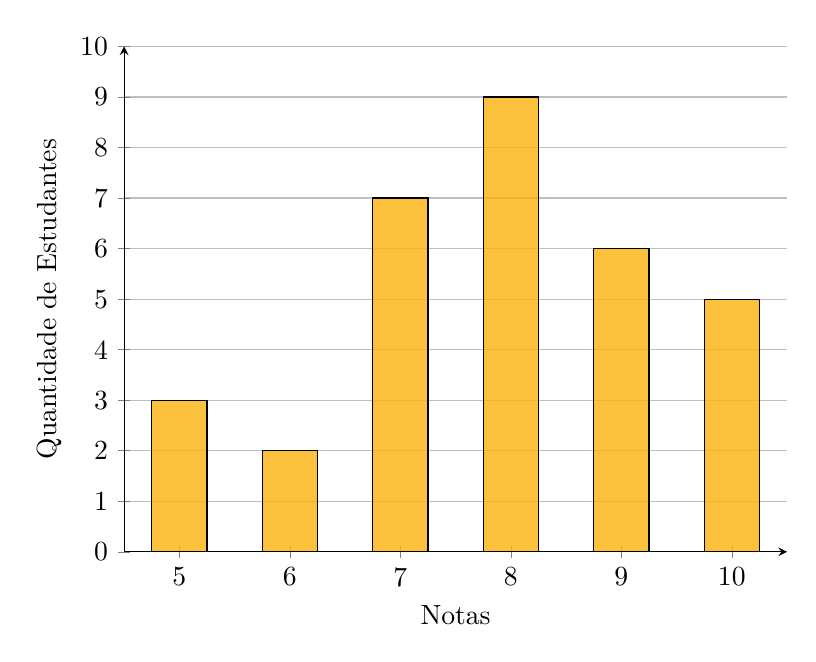
\begin{tikzpicture}
                \begin{axis}[
                        ybar,
                        ytick distance=1,
                        ymax=10,
                        bar width=10pt,
                        xlabel={Notas},
                        ylabel={Quantidade de Estudantes},
                        symbolic x coords={5,6,7,8,9,10},
                        xtick=data,
                        ymin=0,
                        grid=major,
                        xmajorgrids=false,
                        axis lines=left,
                        bar width=20pt,
                        enlarge x limits=0.1,
                        width=10cm,
                        height=8cm,
                    ]
                    \addplot[
                        fill=yellow!40!orange,
                        fill opacity=.8
                    ] coordinates{
                        (5,3) (6,2) (7,7) (8,9) (9,6) (10,5)
                    };
                \end{axis}
            \end{tikzpicture}
        \end{center}

        Quantos estudantes participaram dessa avaliação?

        \begin{multicols}{2}
            \begin{enumerate}[label=\alph*)]
                \item 30 Estudantes
                \item 35 Estudantes
                \item 32 Estudantes
                \item 33 Estudantes
            \end{enumerate}
        \end{multicols}

\begin{solucoes}{1}
    \solucao

    De acordo com o gráfico, temos o valor das notas no eixo horizontal e a quantidade de alunos no eixo vertical, então para saber a quantidade total de estudantes que participaram nessa avaliação, somamos a quantidade de estudantes em cada nota obtida, assim temos:

$\begin{WithArrows}[tikz={>=stealth, text width = 6cm, draw=black!70, text=black!70}, interline=2mm]
    nota\, 5 :&\, 3\, estudantes \\
    nota\, 6 :&\, 2\, estudantes \\
    nota\, 7 :&\, 7\, estudantes \\
    nota\, 8 :&\, 9\, estudantes \\
    nota\, 9 :&\, 6\, estudantes \\
    nota\, 10:&\, 5\, estudantes \\ \hline
              &\, 32\, estudantes
\end{WithArrows}$

Sendo assim, \textbf{32 estudantes} realizaram à ultima avaliação do professor Tony.

\textbf{ALTERNATIVA C}
\end{solucoes}

\section{Grandezas e Medidas}

\questao{Primeira questão}



% Questões do 8° ano

\chapter{8$^{\circ}$ Ano}

\begin{caixainfo}

\textbf{Matemática — 8$^{\circ}$ ano}

Neste capítulo estão reunidas questões destinadas ao 8$^{\circ}$ ano do Ensino Fundamental, organizadas de acordo com as Unidades Temáticas da BNCC.

\end{caixainfo}

\vspace{1cm}

\section*{Unidades Temáticas}

\begin{center}

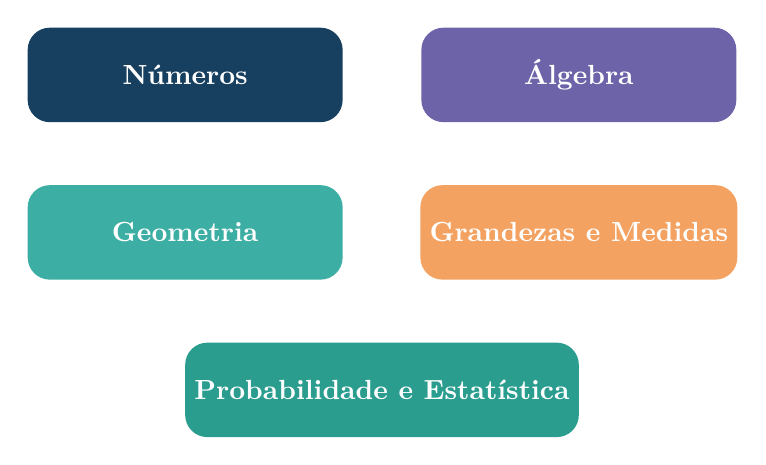
\begin{tikzpicture}

\node[
    rounded corners=8pt,
    fill=AzulPrincipal,
    text=white,
    minimum width=4cm,
    minimum height=1.2cm
] (n) at (0,0) {\textbf{Números}};

\node[
    rounded corners=8pt,
    fill=Roxo,
    text=white,
    minimum width=4cm,
    minimum height=1.2cm
] (a) at (5,0) {\textbf{Álgebra}};

\node[
    rounded corners=8pt,
    fill=Turquesa,
    text=white,
    minimum width=4cm,
    minimum height=1.2cm
] (g) at (0,-2) {\textbf{Geometria}};

\node[
    rounded corners=8pt,
    fill=Laranja,
    text=white,
    minimum width=4cm,
    minimum height=1.2cm
] (m) at (5,-2) {\textbf{Grandezas e Medidas}};

\node[
    rounded corners=8pt,
    fill=Verde,
    text=white,
    minimum width=4cm,
    minimum height=1.2cm
] (p) at (2.5,-4) {\textbf{Probabilidade e Estatística}};

\end{tikzpicture}

\end{center}

\clearpage


\section{Números}

\questao{Primeira questão}


\section{Álgebra}

\questao{(OM$^3$SP 2026 - 1ª Fase) Em um dia ensolarado Aldemir, coordenador dos Anos Iniciais, propôs um desafio matemático com as letras $M$ e $P$ que compõem a logo da escola. Ele associou essas letras a dois algarismos, do $0$ ao $9$, e escreveu em uma painel da escola que $MP+PM=121$ e $PM-PP=1$. Qual será o valor numérico encontrado para  $M$?}
        \begin{multicols}{4}
                \begin{enumerate}[label=\alph*)]
                    \item 5
                    \item 6
                    \item 7
                    \item 8
                \end{enumerate}
            \end{multicols}

\begin{solucoes}{2}
    \solucao
Nesta questão, tem-se que $M$ e $P$ são algarismos, ou seja, estão entre os números inteiro de 0 a 9. Sabe-se também que  $MP+PM=121$ e $PM-PP=1$. Partindo de $MP+PM=121$, tem-se que, para gerar final 1, as opções são $0$ e $1$, $2$ e $9$, $3$ e $8$, $4$ e $7$ ou $5$ e $6$. Olhando para essas opções, a única que será prontamente descartada é $M=0$ e $P=1$, pois $01+10=11\neq 121$. Todas as outras somadas darão $121$. Com isso, é preciso notar que $PM-PP=1$ e, para isso acontecer, $M-P=1$. O único caso possível seria $M=6$ e $P=5$. Sendo assim, $M=6$.\\
\textbf{ALTERNATIVA B}

\solucao

Podemos pensar de outra maneira e, com isso, podemos resolver de uma forma puramente algébrica. Assim, partindo da primeira informação, 
\begin{equation*}
MP+PM=121
\end{equation*}
\begin{equation*}
    (10M+P)+(10P+M)=121
\end{equation*}
\begin{equation*}
    (10M+M)+(10P+P)=121
\end{equation*}
\begin{equation*}
    11M+11P=121
\end{equation*}
\begin{equation*}
    11*(M+P)=121
\end{equation*}
\begin{equation*}
    M+P=\frac{121}{11}=11
\end{equation*}
\begin{equation*}
    M+P=11 \ (1)
\end{equation*}

Faremos a mesma coisa com a segunda informação,

\begin{equation*}
    PM-PP=1
\end{equation*}
\begin{equation*}
    (10P+M)-(10P+P)=1
\end{equation*}
\begin{equation*}
    M-11M+10M=1
\end{equation*}
\begin{equation*}
    M-P=1 \ (2)
\end{equation*}

Somando $(1)$ e $(2)$,temos que

\begin{equation*}
  2M=12
\end{equation*}
\begin{equation*}
    M=\frac{12}{2}=6
\end{equation*}
Com isso, determinamos que $M=6$. \\
\textbf{ALTERNATIVA B}
\end{solucoes}

\questao{(OM$^3$SP 2026 - 1ª Fase) Na última semana, a Vice-Diretora Quitéria saiu ao portão de entrada da E.M.M.M.S.P. e percebeu que tinham alguns carros e algumas motos estacionadas na frente da escola. Ao entrar ela disse a Félix que o número total de automóveis, apenas carros e motos, presentes na frente da escola era de 12. Ela também contou e determinou que a quantidade de rodas era de 34. Com isso, Félix descobriu quantas motos e quantos carros ali estavam. Qual era o número de motos presentes naquele momento na frenta da E.M.M.M.S.P.?}
        \begin{multicols}{4}
                \begin{enumerate}[label=\alph*)]
                    \item 5
                    \item 6
                    \item 7
                    \item 8
                \end{enumerate}
            \end{multicols}

\begin{solucoes}{2}

\solucao
    Tem-se aqui um clássico problema de sistema de equações do primeiro grau. Tome $C$ representando o número de carros e $M$ o número de motos. Convertendo as informações em equações, ter-se-á:
        \begin{equation*}
\begin{cases}
  C+M=12\\
     4C+2M=34 
\end{cases}
 \end{equation*}
    Ao multiplicar por $-4$ a primeira equação. ter-se-á:
        \begin{equation*}
\begin{cases}
    -4C+-4M=-48\\
     4C+2M=34 
\end{cases}
 \end{equation*}   
Somanda asduasequações acima,teremos
\begin{equation*}
    -2M=-14
\end{equation*} 
\begin{equation*}
    M=\frac{14}{2}=7
\end{equation*}
Assim, na porta da escola havia 7 motos.\\
\textbf{ALTERNATIVA C}

\solucao

Podemos resolver este problema de uma forma menos algébrica e mais aritmética. Pense o seguinte, se todos os veículos fossem motos teríamos $12*2=24$, todavia temos $34$ rodas. Sendo assim, temos 10 rodas a mais do que o número de motos e como cada carro possui o dobro de rodas de cada moto, devemos então dividir $\frac{10}{2}=5$. Logo, serão $5$ carros e assim $7$ motos.  \\
\textbf{ALTERNATIVA C}

\end{solucoes}



\section{Geometria}

\questao{(Elaboração própria) Qual a quantidade de quadrados (de qualquer tamanho) que você consegue identificar na figura a seguir?}

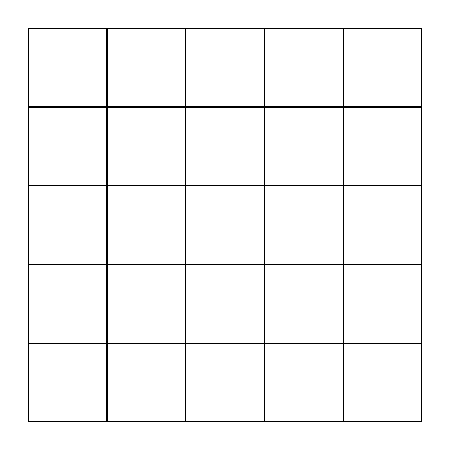
\begin{tikzpicture}
    \foreach \x in {0,1,2,3,4}{
        \foreach \y in {0,1,2,3,4}{
            \draw(\x,\y) rectangle ++(1,1);
        }
    }
\end{tikzpicture}

\begin{multicols}{4}
    \begin{enumerate}[label=\alph*)]
        \item 25
        \item 40
        \item 30
        \item 55
    \end{enumerate}
\end{multicols}

\begin{solucoes}{2}
    \solucao 

    Se considermos seguir a logica de contar cada quadrado, teremos, 25 quadradinhos 1x1, 16 quadradinhos 2x2, 9 quadrados 3x3, 4 quadrados 4x4 e 1 quadrado 5x5, assim, ficamos com a seguinte soma:

    $$25 + 16 + 9 + 4 + 1 = 55\,\, \text{Quadrados}$$

    \textbf{ALTERNATIVA D}

    \solucao

    Uma outra forma de resolver essa questão, é utilizar a formula da soma dos quadrados do enésimo termo.

    $$1^{2} + 2^{2} + 3^{2} + \cdots + n^{2} = \cfrac{n\cdot(n+1)\cdot(2n+1)}{6}$$

    Assim, ja que temos um quadrado 5x5, formado por quadradinhos 1x1, obtemos a seguinte operação:

    $$\cfrac{5\cdot(5+1)\cdot(2\cdot5+1)}{6} = \cfrac{5\cdot6\cdot11}{6} = \cfrac{5\cdot\canceldiv{6}{6}\cdot11}{\canceldiv{6}{6}} = 5\cdot11= 55 \,\, \text{quadrados totais}$$

    \textbf{ALTERNATIVA D}
\end{solucoes}
\section{Probabilidade e Estatística}

\questao{O quadriculado $3\times3$ preenchido com números inteiros recebe o nome de medmágico quando, em cada linha horizontal, vertical ou diagonal, o número central funciona como a média aritmética dos dois números que estão nas extremidades.}

        \begin{flushright}
            {\renewcommand{\arraystretch}{1.5}
            \begin{tabular}{
                |>{\centering\arraybackslash}m{.5cm}|>{\centering\arraybackslash}m{.5cm}|>{\centering\arraybackslash}m{.5cm}|
                }
                 \hline
                 11& 15 & 19 \\\hline
                 6 & 10 & 14\\ \hline
                 1 & 5  & 9\\ \hline
            \end{tabular}}
        \end{flushright}

        \begin{enumerate}[label=\alph*)]
            \item Preencha o quadriculado abaixo para que ele seja medmágico.
            \vspace{10pt}
           
            {\renewcommand{\arraystretch}{1.5}
            \begin{tabular}{
                |>{\centering\arraybackslash}m{.5cm}|>{\centering\arraybackslash}m{.5cm}|>{\centering\arraybackslash}m{.5cm}|
                }
                 \hline
                 4&  & 18 \\\hline
                 8&  & \\ \hline
                  &  & \\ \hline
            \end{tabular}}

            \vspace{1cm}

            \item Em um quadriculado medmágico $3\times3$, os números 9, 8 e 25 ocupam as posições mostradas na figura. Determine o valor de x.

            
            {\renewcommand{\arraystretch}{1.5}
            \begin{tabular}{
                |>{\centering\arraybackslash}p{.5cm}|>{\centering\arraybackslash}p{.5cm}|>{\centering\arraybackslash}p{.5cm}|
                }
                 \hline
                 & 9 &  \\\hline
                 8& x & \\ \hline
                  &  & 25\\ \hline
            \end{tabular}}

            \vspace{1cm}

            \item Justifique por que, em qualquer quadriculado medmágico, a soma dos nove valores sempre resulta em um múltiplo de 9.

        \end{enumerate}

\begin{solucoes}{1}
    \solucao
    \textbf{item a)}

\begin{figure}[H]
    \begin{minipage}{.7\linewidth}
        Para facilitar, colocamos letras nas casas vazias:

        O número a deve ser a média dos números 3 e 19:
    \end{minipage}
    \begin{minipage}{.25\linewidth}
        {\renewcommand{\arraystretch}{1.5}
            \begin{tabular}{
                |>{\centering\arraybackslash}m{.5cm}|>{\centering\arraybackslash}m{.5cm}|>{\centering\arraybackslash}m{.5cm}|
                }
                 \hline
                 4& a & 18 \\\hline
                 8& c & d\\ \hline
                 b & e & f\\ \hline
            \end{tabular}}
    \end{minipage}
\end{figure}

$a = \cfrac{4+18}{2} = 11$

O número 8 deve ser a média entre 4 e b, ou seja:

$\cfrac{4+b}{2} = 8 \Rightarrow 4 + b = 8\times2 \Rightarrow b = 16 - 4 \Rightarrow b = 12$ 

Logo, $b = 12$

O número c deve ser a média entre 18 e 12: $c = \cfrac{18+12}{2} \Rightarrow c = \cfrac{30}{2} \Rightarrow c = 15$

{\renewcommand{\arraystretch}{1.5}
\begin{tabular}{
    |>{\centering\arraybackslash}m{.5cm}|>{\centering\arraybackslash}m{.5cm}|>{\centering\arraybackslash}m{.5cm}|
    }
     \hline
     4& \textbf{11} & 18 \\\hline
     8& \textbf{15} & d\\ \hline
     \textbf{12} & e & f\\ \hline
\end{tabular}}

\vspace{20pt}

Analogamente,

$
\begin{cases}
    \cfrac{d + 8}{2} = 15 \Rightarrow d + 8 = 30 \Rightarrow d = 22\\
    \cfrac{e + 11}{2}=15 \Rightarrow e + 11 = 30 \Rightarrow e = 19\\
    \cfrac{f + 4}{2} = 15 \Rightarrow f + 4 = 30 \Rightarrow f = 26
\end{cases}$

Portanto, o preenchimento final do quadriculado medmágico é:

{\renewcommand{\arraystretch}{1.5}
\begin{tabular}{
    |>{\centering\arraybackslash}m{.5cm}|>{\centering\arraybackslash}m{.5cm}|>{\centering\arraybackslash}m{.5cm}|
    }
     \hline
     4& \textbf{11} & 18 \\\hline
     8& \textbf{15} & \textbf{22}\\ \hline
     \textbf{12} & \textbf{19} & \textbf{26}\\ \hline
\end{tabular}}

\solucao

\textbf{item b)}

Primeiramente, colocamos letras nas casas vazias, de acordo com a figura abaixo:

{\renewcommand{\arraystretch}{1.5}
\begin{tabular}{
    |>{\centering\arraybackslash}p{.5cm}|>{\centering\arraybackslash}p{.5cm}|>{\centering\arraybackslash}p{.5cm}|
    }
     \hline
     y& 9 &v  \\\hline
     8& x & w\\ \hline
      t& z & 25\\ \hline
\end{tabular}}

Calculando as médias, obtemos:

$\begin{cases}
    \cfrac{y+25}{2} = x \Rightarrow y + 25 = 2x \Rightarrow y = 2x - 25\\
    \cfrac{z + 9}{2} = x \Rightarrow z + 9 = 2x \Rightarrow z = 2x - 9\\
    \cfrac{w + 8}{2} = x \Rightarrow w + 8 = 2x \Rightarrow w = 2x - 8
\end{cases}$

Isso nos permite também calcular v e t em função de x:

{\renewcommand{\arraystretch}{1.5}
\begin{tabular}{
    |>{\centering\arraybackslash}m{1.25cm}|>{\centering\arraybackslash}m{.9cm}|>{\centering\arraybackslash}m{.9cm}|
    }
     \hline
     2x-25& 9 &v  \\\hline
     8& x & 2x-8\\ \hline
      t& 2x-9 & 25\\ \hline
\end{tabular}}

$\begin{cases}
    \cfrac{v+25}{2} = 2x-8 \Rightarrow v + 25 = 4x-16 \Rightarrow v = 4x - 41\\
    \cfrac{t+2x-25}{2} = 8 \Rightarrow t + 2x - 25 = 16 \Rightarrow t = -2x + 41
\end{cases}$

{\renewcommand{\arraystretch}{1.5}
\begin{tabular}{
    |>{\centering\arraybackslash}m{1.5cm}|>{\centering\arraybackslash}m{1.5cm}|>{\centering\arraybackslash}m{1.5cm}|
    }
     \hline
     2x-25& 9 &4x - 41  \\\hline
     8& x & 2x-8\\ \hline
      -2x+41& 2x-9 & 25\\ \hline
\end{tabular}}

Segue, da terceira linha do quadriculado acima, que:

$\cfrac{-2x+41+25}{2} = 2x-9 \Rightarrow -2x + 66 = 4x - 18 \Rightarrow 84 = 6x \Rightarrow x = \cfrac{84}{6} \Rightarrow x = 14$

Utilizando esse valor encontrado de x, os outros valores podem ser facilmente
calculados e o preenchimento final do quadriculado medmágico, nesse caso, é:

{\renewcommand{\arraystretch}{1.5}
\begin{tabular}{
    |>{\centering\arraybackslash}m{1.5cm}|>{\centering\arraybackslash}m{1.5cm}|>{\centering\arraybackslash}m{1.5cm}|
    }
     \hline
     3& 9 &15  \\\hline
     8& 14 & 10\\ \hline
      13& 19 & 25\\ \hline
\end{tabular}}

\solucao
\textbf{item c)}

Consideremos agora um quadrado medmágico qualquer, como o da figura abaixo

\begin{figure}[H]
    \begin{minipage}{.3\linewidth}
        \begin{center}
            {\renewcommand{\arraystretch}{1.5}
            \begin{tabular}{
                |>{\centering\arraybackslash}m{.5cm}|>{\centering\arraybackslash}m{.5cm}|>{\centering\arraybackslash}m{.5cm}|
                }
                 \hline
                 a& b &c  \\\hline
                 d& e & f\\ \hline
                  g& h & i\\ \hline
            \end{tabular}}
        \end{center}
    \end{minipage} $\Rightarrow$
    \begin{minipage}{.3\linewidth}
        $\begin{cases}
            a + i = 2e \\
            b + h = 2e \\ 
            c + g = 2e \\
            d + f = 2e
        \end{cases}$
    \end{minipage}
\end{figure}

$\Rightarrow$ a + b + c + d + e + f + g + h + i = 2e + 2e + 2e + 2e + e = 9e

Como o número representado pela letra \underline{e} é um número inteiro, a soma de todos é múltipla de 9.

Concluímos assim que em qualquer quadriculado medmágico a soma de todos os seus números é igual a 9 vezes o
termo central.

\end{solucoes}
\section{Grandezas e Medidas}

\questao{Primeira questão}


% Questões do 9° ano

\chapter{9$^{\circ}$ Ano}

\begin{caixainfo}

\textbf{Matemática — 9$^{\circ}$ ano}

Neste capítulo estão reunidas questões destinadas ao 9$^{\circ}$ ano do Ensino Fundamental, organizadas de acordo com as Unidades Temáticas da BNCC.

\end{caixainfo}

\vspace{1cm}

\section*{Unidades Temáticas}

\begin{center}

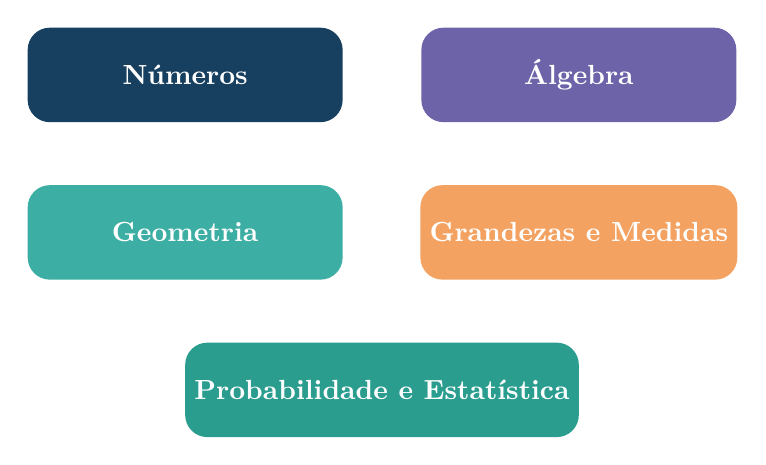
\begin{tikzpicture}

\node[
    rounded corners=8pt,
    fill=AzulPrincipal,
    text=white,
    minimum width=4cm,
    minimum height=1.2cm
] (n) at (0,0) {\textbf{Números}};

\node[
    rounded corners=8pt,
    fill=Roxo,
    text=white,
    minimum width=4cm,
    minimum height=1.2cm
] (a) at (5,0) {\textbf{Álgebra}};

\node[
    rounded corners=8pt,
    fill=Turquesa,
    text=white,
    minimum width=4cm,
    minimum height=1.2cm
] (g) at (0,-2) {\textbf{Geometria}};

\node[
    rounded corners=8pt,
    fill=Laranja,
    text=white,
    minimum width=4cm,
    minimum height=1.2cm
] (m) at (5,-2) {\textbf{Grandezas e Medidas}};

\node[
    rounded corners=8pt,
    fill=Verde,
    text=white,
    minimum width=4cm,
    minimum height=1.2cm
] (p) at (2.5,-4) {\textbf{Probabilidade e Estatística}};

\end{tikzpicture}

\end{center}

\clearpage


\section{Números}

\questao{dfjsiodjfi}

\section{Álgebra}

\questao{(OM$^3$SP 2026 - 1ª Fase) Roberta tem uma loja de roupas que trabalha exclusivamente com camisas. Ela vende todas as camisas por um mesmo preço, todas custam $R\$ \ 40,00$, e vendia cerca de $20$ camisas por dia. Ela fez uma promoção e percebeu que a cada $R\$ \ 1,00$ de desconto ela vendia $10$ camisas a mais. Qual será o valor da camisa para que Roberta tenha o faturamento máximo?}
         \begin{multicols}{4}
            \begin{enumerate}[label=\alph*)]
                \item $21$
                \item $28$
                \item $36$
                \item $45$
            \end{enumerate}
        \end{multicols}

\begin{solucoes}{1}
    \solucao
Tome como $x$ como o valor do desconto. Considere $P(x)$ a função que representa o preço e $Q(x)$ a função que representa a quantidade. Assim, teremos:
        \begin{equation*}
            V(x)=P(x)\cdot Q(x)
        \end{equation*}
            \begin{equation*}
            V(x)=(40-x)(20+10x)
        \end{equation*}
          \begin{equation*}
            V(x)=-10x^2+380x+800
        \end{equation*}
        Para haver faturamento máximo, $x_v=\frac{-b}{2\cdot a}=\frac{-380}{2\cdot (-10
        )}=\frac{-380}{-20}=19$. Sendo assim, como $x=19$, o novo valor da camisa será de $40-19=21$.\\
        \textbf{ALTERNATIVA A}
\end{solucoes}

\questao{(Elaboração própria) O Professor Samuel afirmou que $p$ é um número primo, e p$\geq5$, o valor da expressão algébrica $p^2 - 1$ será sempre um múltiplo de qual dos números abaixo?}

\begin{multicols}{4}
    \begin{enumerate}[label=\alph*) ]
        \item 10
        \item 24
        \item 13
        \item 19
    \end{enumerate}
\end{multicols}
\begin{solucoes}{2}
    \solucao
    \textbf{Testando valores} temos, como a questão afirmar que a regra vale para qualquer número primo, maior ou igual a 5,  só precisamos testar o primeiro valor número que se encaixa nessa regra para eliminar as alternativas incorretas.

    Primeiro, escolhemos o menor número primo maior ou igual a 5, que no caso é o próprio 5.

    Substituindo na expressão, temos:

    $$p^2-1 = 5^2 - 1 = 25 -1 = 24$$

    Analisando as alternativas, o 24 não é múltiplo do 10, nem do 13 e nem do 19, sendo apenas múltiplo do próprio 24. Assim, já resolvemos a questão.

    Porem, para ter certeza, vamos testar para o próximo número primeiro depois do 5, usando o 7.

    Temos o seguinte resultado:

    $$7^2 - 1 = 49 -1 = 48$$

    como 48 é 24 $\times$ 2, ele também é um múltiplo de 24, confirmando a regra.

    \textbf{ALTERNATIVA B}

    \solucao

    \textbf{Demonstração algébrica}, podemos utilizar também os produtos notáveis para realizar a solução dessa questão.

    Temos que:

    $$p^2 - 1 = (p+1)(p-1)$$

    e como \textbf{p} é um número primo maior que 2, então ele é impar. Logo (p-1) e (p+1) são dois números pares consecutivos, exemplo, se p = 7, teremos 6 e 8.\\

    Sempre que multiplicamos dois pares consecutivos, um deles obrigatoriamente é múltiplo de 2 e o outro é múltiplo de 4 e a multiplicação deles garantem que o resultado seja um múltiplo de 2 $\times$ 4 = 8. Assim, garantimos a divisibilidade por 8.\\

    para garantir a divisibilidade por 3, temos que em qualquer sequencia  de três números consecutivos como (p-1), p, (p+1), obrigatoriamente um deles é múltiplo de 3. \\

    Como p é primo maior que 3, o próprio p não pode ser múltiplo de 3, assim, (p-1) ou (p+1) será múltiplo de 3.\\

    Se a multiplicação de (p-1)(p+1) é divisível por 8 e também por 3, então obrigatoriamente tem que ser divisível  por 3 $\times$ 8 = 24.

    \textbf{ALTERNATIVA B}
\end{solucoes}

\section{Geometria}

\questao{(OM$^3$SP 2026 - 1ª Fase) O professor Genílson estava fazendo uma obra em casa e usou sua grande escada para auxiliar na pintura superior de sua parede. Sabe-se que a distância da base da escada até a parede mede $12 m$. Ele também sabe que a escada tem $13m$ de comprimento. A que altura esta escada se encontra do chão?}
        \begin{multicols}{4}
            \begin{enumerate}[label=\alph*)]
                \item $4m$
                \item $5m$
                \item $6m$
                \item $7m$
        \end{enumerate}
        \end{multicols}

\begin{solucoes}{1}
    \solucao
    No problema do professor Genilson se tem a situação a seguir,
        \begin{figure}[H]
            \centering
            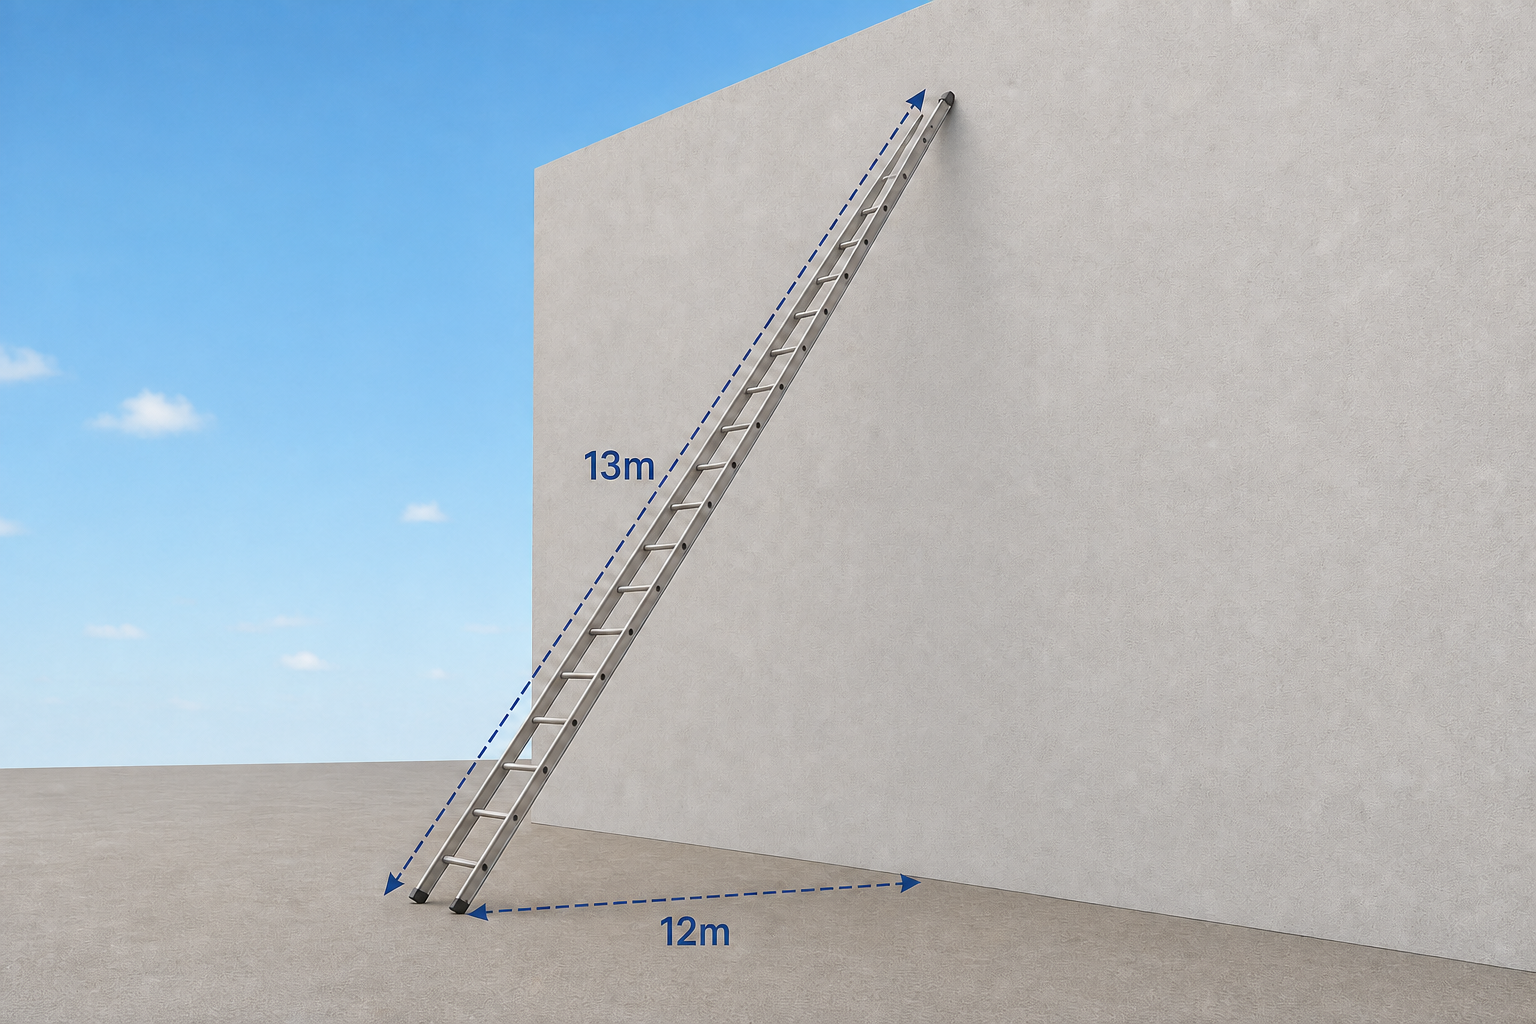
\includegraphics[width=0.5\linewidth]{figuras/9_ano/IMG_0937.png}
        \end{figure}
        Como o triângulo gerado é retângulo, pode-se utilizar o teorema de Pitágoras. Com isso, 
        \begin{equation*}
            13^2=12^2+x^2
        \end{equation*}
        \begin{equation*}
            169=144+x^2
        \end{equation*}
        \begin{equation*}
           x^2=169-144
        \end{equation*}
        \begin{equation*}
         x^2=25
        \end{equation*}
        \begin{equation*}
            x=\sqrt{25}=5
        \end{equation*}
        Sendo assim, a altura da escada até o chão é de $5m$.\\
        \textbf{ALTERNATIVA B}
\end{solucoes}

\questao{(OM$^3$SP 2026 - 1ª Fase) A professora Elielma acabou de comprar uma mansão e na sala de estar de sua mansão, existe uma escada em formato de caracol (espiral) ligando o andar térreo ao andar superior, conforme mostra à imagem a seguir:}
          \begin{figure}[H]
            \centering
            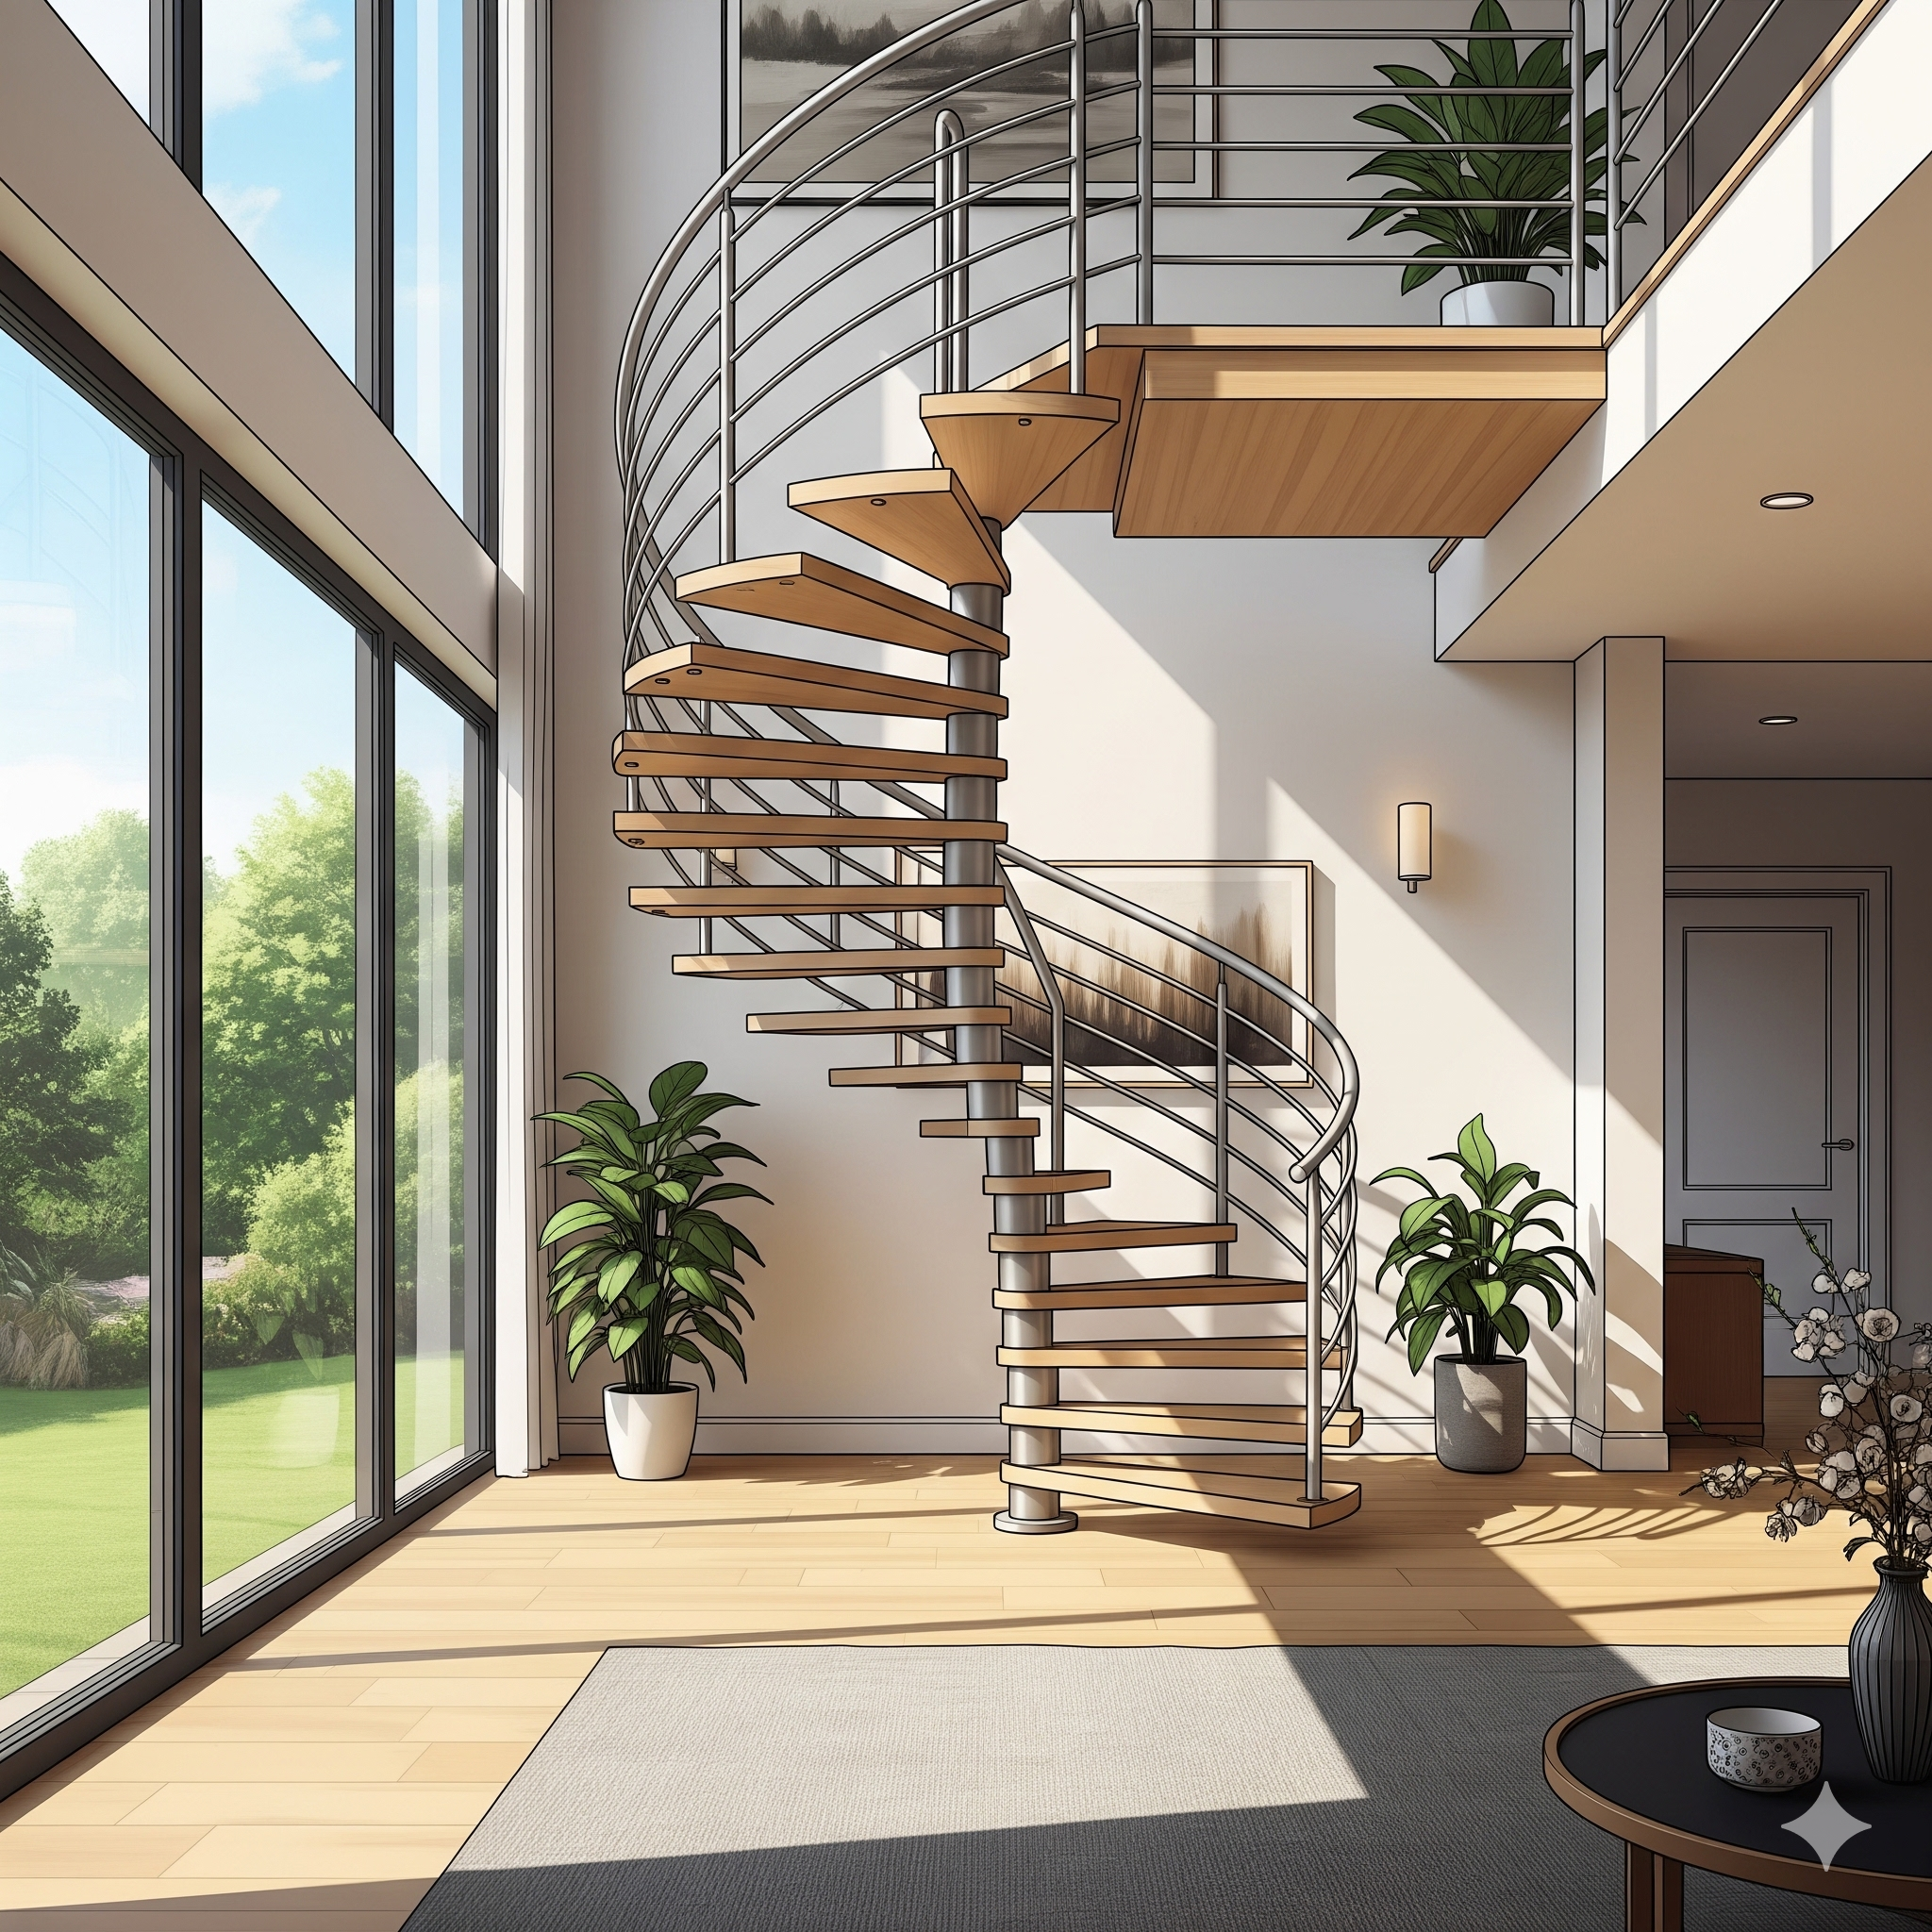
\includegraphics[width=0.4\linewidth]{figuras/9_ano/Escada.png}
        \end{figure}
        A professora Elielma sobe essa escada pisando na ponta de cada degrau para chegar ao seu quarto. Ao meio-dia, o sol está a pino e seus raios de luz incidem de forma perfeitamente perpendicular (formando um ângulo de 90°) em relação ao chão plano da sala. Qual figura geométrica plana o desenho da sombra gerada formaria?
        \begin{multicols}{4}
            \begin{enumerate}[label=\alph*)]
                \item Uma espiral
                \item um retângulo
                \item um círculo
                \item uma reta
            \end{enumerate}
        \end{multicols}

\begin{solucoes}{1}
    \solucao

Nesta imagem, ao olharmos de cima veremos uma figura interessante,
        \begin{figure}[H]
            \centering
            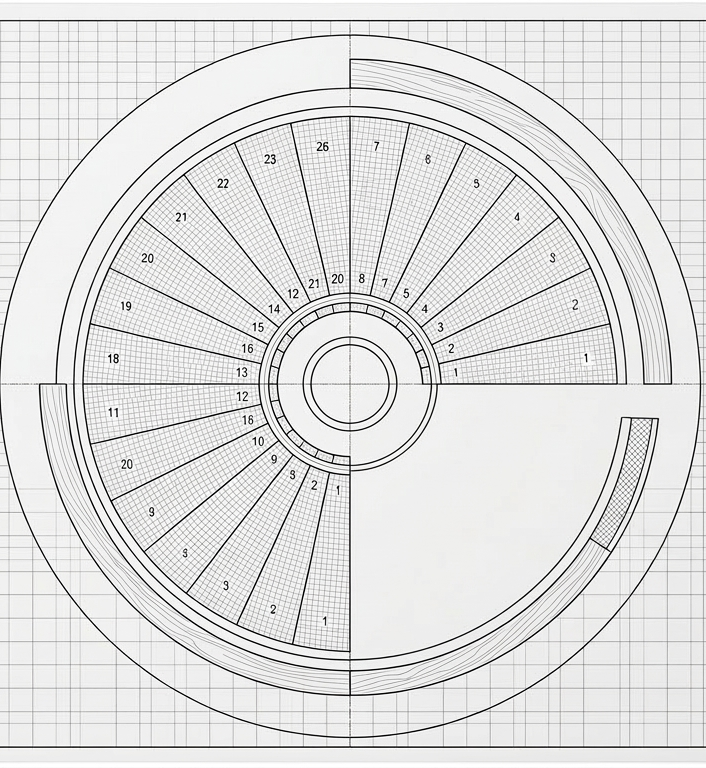
\includegraphics[width=0.4\linewidth]{figuras/9_ano/Projeção.png}
        \end{figure}
        Logo, a projeção ortogonal é dada por um círculo.\\
        \textbf{ALTERNATIVA C}
\end{solucoes}

\questao{(AUTORIA PRÓPRIA) Mostre que em um triângulo pitagórico, triângulo retângulo de lados inteiros, primitivo, o $mdc(x,y,z)=1$, os catetos possuem paridade diferente.}

\begin{solucoes}{1}
\solucao
Dizer que os catetos possuem paridade diferente é o mesmo que dizer que um deles deve ser par e o outro deve ser ímpar. Considere um triângulo pitagórico primitivo de lados $x,y$ e $z$, onde $x^2+y^2=z^2$ ($x$ e $y$ são os catetos e $z$ a hipotenusa) e $mdc(x,y,z)=1$. Para concluírmos o que se pede é preciso lembrar que só existem três possibilidades, ambos pares, ambos ímpares e terem paridade diferente. Mostremos por contradição que não podem ser ou ambos pares ou ambos ímpares,  

$i)$ Se ambos forem pares teríamos $x=2k$ e $y=2l$. Assim, 
\begin{equation*}
    x^2+y^2=(2k)^2+(2l)^2=4(k^2+l^2)=4p=z^2
\end{equation*}
O que é uma contradição, pois assim $z^2=$ é um múltiplo de 4 e $z$ é múltiplo de 2, o que não pode ocorrer,pois $mdc(x,y,z)=1$. Logo, $x$ e $y$ não podem ser ambos pares.

$ii)$ Se ambos forem ímpares teríamos $x=2k+1$ e $y=2l+1$ (Perceba que dizer que um número é ímpar é o mesmo que dizer que ele deixa resto $1$ quando dividido por $2$ ). Assim, 
\begin{equation*}
    x^2+y^2=(2k+1)^2+(2l+1)^2
\end{equation*}
\begin{equation*}
    x^2+y^2=4k^2+4k+1+4l^2+4l+1=4(k^2+k+l^2+l)+2=4t+2=2(2t+1)=2p
\end{equation*}
Logo, duas coisas saltam aos olhos. Em primeiro lugar, mostramos que a soma do quadrado de dois números ímpares deixa resto $2$ na divisão por quatro e em segundo lugar, mostramos que $z^2$ é par e consequentemente $z=2r$ (deixa resto $0$ na divisão por $2$). Todavia, a segunda informação gera uma contradição, pois $x^2+y^2$ deixa resto $2$ na divisão por 4 e $z^2=(2r)^2=4r^2$ e sendo assim, deixaria resto $0$ na divisão por $4$. Logo, ambos não podem ser ímpares.


Portanto, como ambos não podem ser nem pares e nem ímpares, os catetos de um triângulo pitagórico primitivo possuem paridadesdiferentes.
\end{solucoes}


        
\section{Probabilidade e Estatística}

\questao{Primeira questão}

\section{Grandezas e Medidas}

\questao{Primeira questão}




\end{document}